\section{Utente Autenticato}

Di seguito vengono elencati i \glossaryItem{casi d'uso} per l'utente autenticato.
\subsection{Casi d'Uso}

\subsubsection{Operazioni dell'utente autenticato}

    \begin{figure}[H]
      \begin{center}
        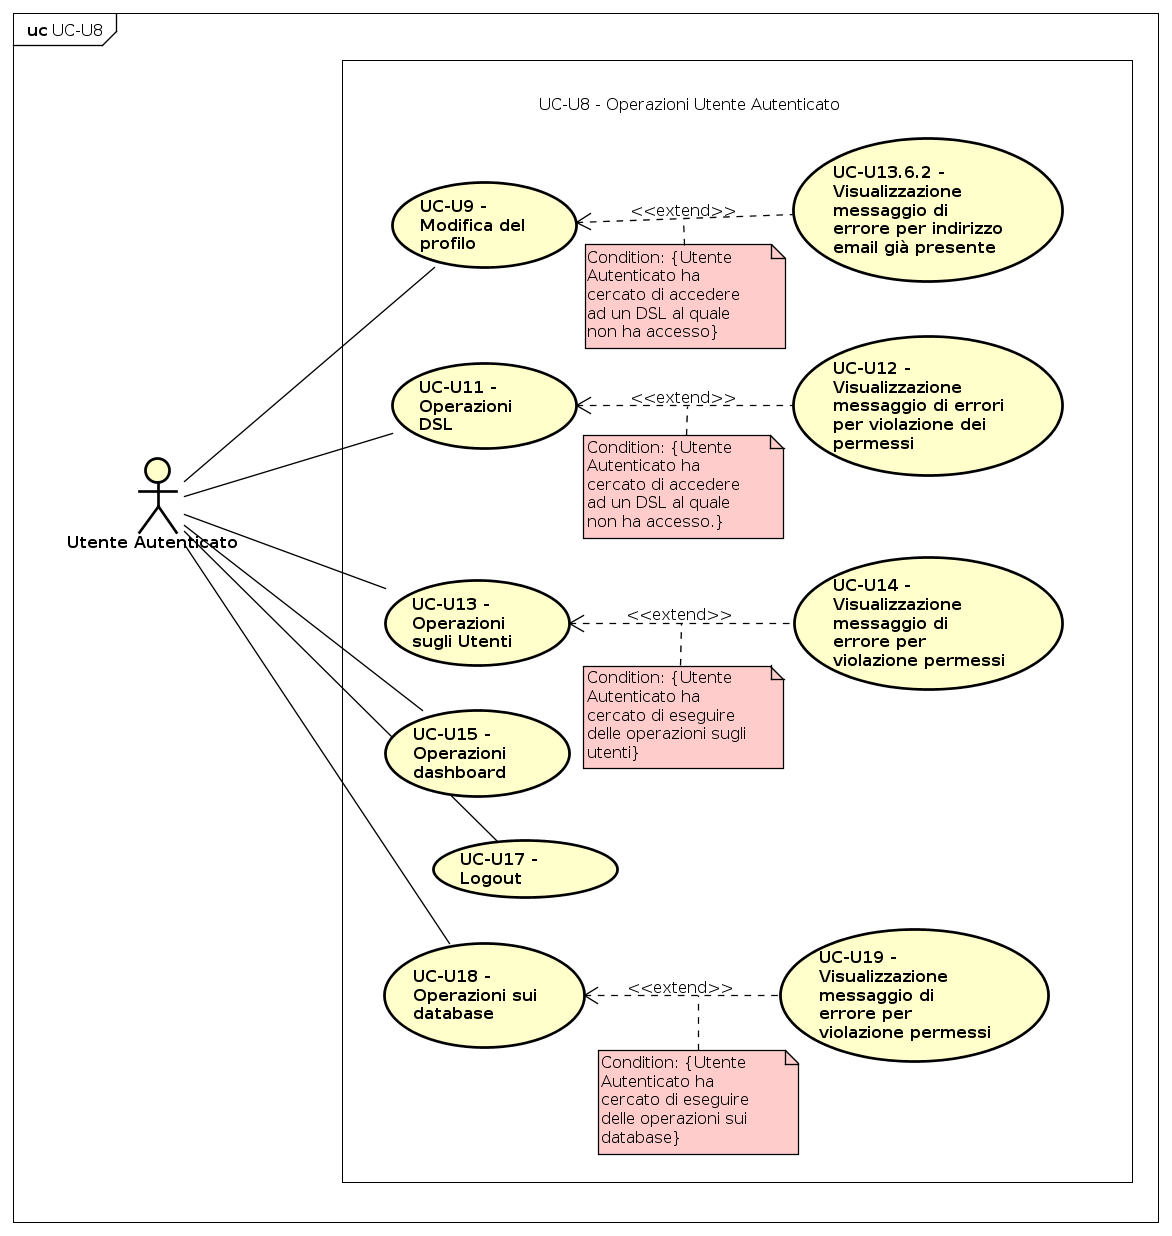
\includegraphics[width=12cm]{res/img/UCUtenti/UCUtenteA/UC-U8.png}
      \caption{UC-U8 - Operazioni dell'utente autenticato}
      \end{center} 
    \end{figure}    
    
    %Tabella 
    \begin{center}
      \bgroup
      \def\arraystretch{1.8}     
      \begin{longtable}{  p{3.5cm} | p{8cm} } 
        
        \hline
        \multicolumn{2}{ | c | }{ \cellcolor[gray]{0.9} \textbf{UC-U8 - Operazioni dell'utente autenticato}} \\ 
        \hline
        
        \textbf{Attori Primari} & Utente autenticato \\ 
        \textbf{Scopo e Descrizione} & L’utente autenticato può: modificare il proprio profilo, effettuare delle operazioni nella pagina \glossaryItem{Dashboard}, effettuare delle operazioni di creazione/modifica/esecuzione delle specifiche DSL (a seconda dei suoi permessi) e gestire altri utenti (quest'ultima funzionalità è riservata ad un ruolo superiore o uguale all'admin). \\ 
        
        \textbf{Precondizioni}  & L’applicazione è funzionante e pronta all'uso. L'utente autenticato ha visualizzato la
        pagina \glossaryItem{Dashboard}. \\ 
        
        \textbf{Postcondizioni} & L'applicazione ha eseguito le azioni richieste dall'utente. \\ 
        \textbf{Scenario principale} & 1. L'utente modifica il proprio profilo. (UC-U9)
        
2. L'utente effettua delle operazioni nella pagina \glossaryItem{Dashboard}. (UC-U15)

3. L'utente effettua delle operazioni di creazione/modifica/esecuzione delle specifiche DSL (a seconda dei suoi permessi). (UC-U11)

4. L'utente gestisce altri utenti (quest'ultima funzionalità è riservata ad un ruolo superiore o uguale all'admin). (UC-U13)

5. L'utente effettua il logout. (UC-U17)

6. L'utente gestisce i database della Company. (UC-U18)  \\
        \textbf{Estensioni} & 1. L'utente autenticato visualizza un messaggio di errore nella procedura di modifica del profilo dovuto all'inserimento di un indirizzo email già presente (UC-U13.6.2)
        
2. L'utente autenticato visualizza un messaggio di errore durante le operazioni effettuate sulle specifiche DSL dovuto alla violazione dei permessi. (UC-U12)

3. L'utente autenticato visualizza un messaggio di errore durante le operazioni sugli utenti dovute alla violazione dei permessi. (UC-U14)

4. L'utente autenticato visualizza un messaggio di errore durante la gestione dei database dovute alla violazione dei permessi. (UC-U19) \\
      \end{longtable}
      \egroup
    \end{center} 


\subsubsection{Operazioni sul profilo}

    \begin{figure}[H]
      \begin{center}
        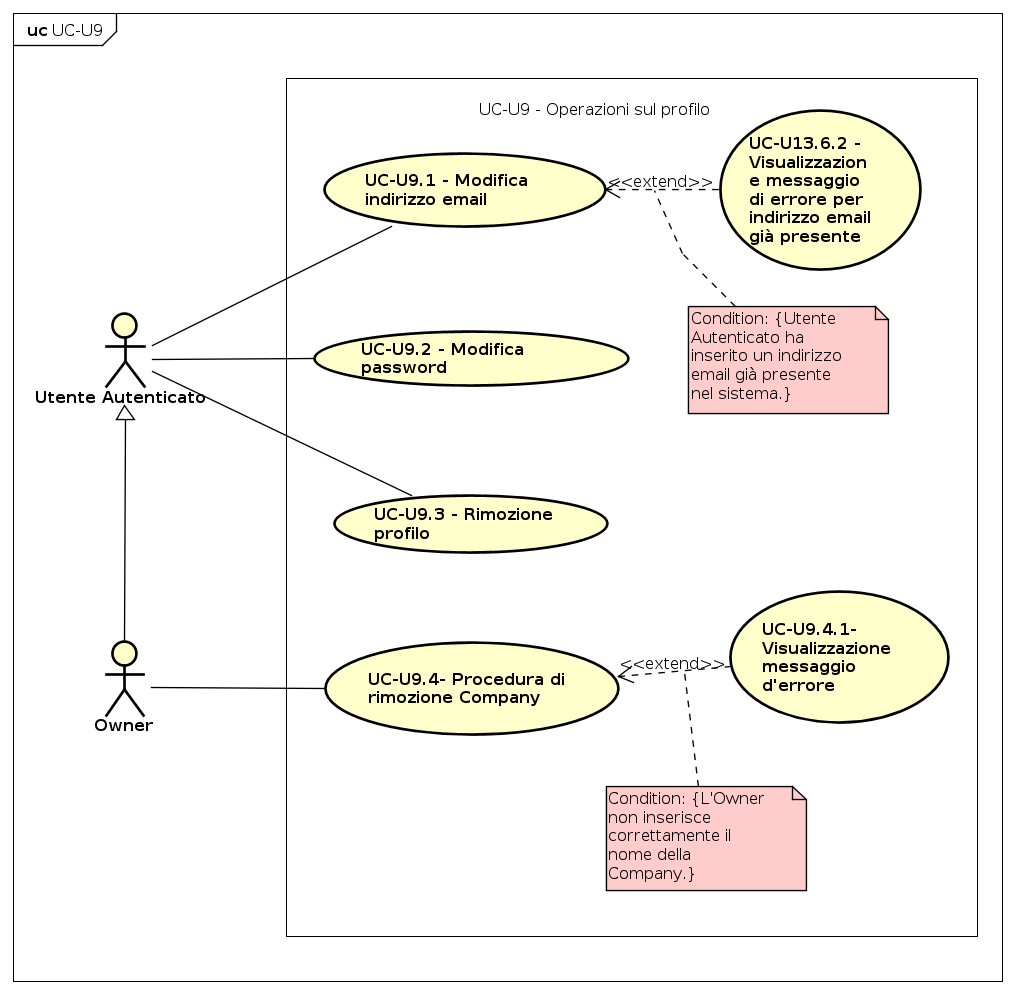
\includegraphics[width=12cm]{res/img/UCUtenti/UCUtenteA/UC-U9- Operazioni sul profilo/UC-U9.png}
      \caption{UC-U9 - Operazioni sul profilo}
      \end{center} 
    \end{figure}    
    
    %Tabella 
    \begin{center}
      \bgroup
      \def\arraystretch{1.8}     
      \begin{longtable}{  p{3.5cm} | p{8cm} } 
        
        \hline
        \multicolumn{2}{ | c | }{ \cellcolor[gray]{0.9} \textbf{UC-U9 - Operazioni sul profilo}} \\ 
        \hline
        
        \textbf{Attori Primari} & Utente autenticato \\ 
        \textbf{Scopo e Descrizione} & L'utente autenticato visualizza la pagina per apportare modifiche al profilo personale. Può decidere di: modificare l'indirizzo email (l'indirizzo e-mail è modificabile in quanto, sebbene unico, non identifica univocamente un utente all'interno dell'applicazione. L'identificazione viene fatta tramite un ID), la password, o rimuovere il profilo.  \\ 
        %1) The professor says: the 'email' field is one of the system's identifier element, thus it shouldn't be modified
        \textbf{Precondizioni}  & L’applicazione è funzionante e pronta all'uso. L'utente autenticato ha visualizzato la
        pagina \glossaryItem{Dashboard}. \\ 
        
        \textbf{Postcondizioni} & Le (eventuali) modifiche del profilo richieste dall'utente sono state apportate. \\ 
        \textbf{Scenario principale} & 1. L'utente autenticato modifica il proprio indirizzo email. (UC-U9.1)
        
2. L'utente autenticato modifica la propria password. (UC-U9.2)

3. L'utente autenticato rimuove il suo profilo/account. (UC-U9.3)

4. L'\textit{Owner} rimuove la propria \textit{Company} (UC-U9.4) \\
\textbf{Estensioni} & 1. L'utente visualizza un messaggio di errore durante la modifica dell'email dovuto all'inserimento di un indirizzo email già presente. (UC-U13.6.2) \\
      \end{longtable}
      \egroup
    \end{center} 

\subsubsection{Modifica indirizzo email}

    %Tabella 
    \begin{center}
      \bgroup
      \def\arraystretch{1.8}     
      \begin{longtable}{  p{3.5cm} | p{8cm} } 
        
        \hline
        \multicolumn{2}{ | c | }{ \cellcolor[gray]{0.9} \textbf{UC-U9.1 - Modifica indirizzo email}} \\ 
        \hline
        
        \textbf{Attori Primari} & Utente autenticato \\ 
        \textbf{Scopo e Descrizione} & L'utente autenticato può modificare il proprio indirizzo email. \\ 
        
        \textbf{Precondizioni}  & L'utente autenticato ha visualizzato la pagina di modifica del profilo. \\ 
        
        \textbf{Postcondizioni} & Il sistema registra un nuovo indirizzo email per il profilo dell'utente autenticato. \\ 
        \textbf{Scenario principale} & 1. L'utente autenticato può modificare il proprio indirizzo email. \\
        \textbf{Estensioni} & 1. L'utente visualizza un messaggio di errore durante la modifica dell'email dovuto all'inserimento di un indirizzo email già presente. (UC-U13.6.2) \\
      \end{longtable}
      \egroup
    \end{center}
    
    
\subsubsection{Modifica password}
 

    \begin{figure}[H]
      \begin{center}
        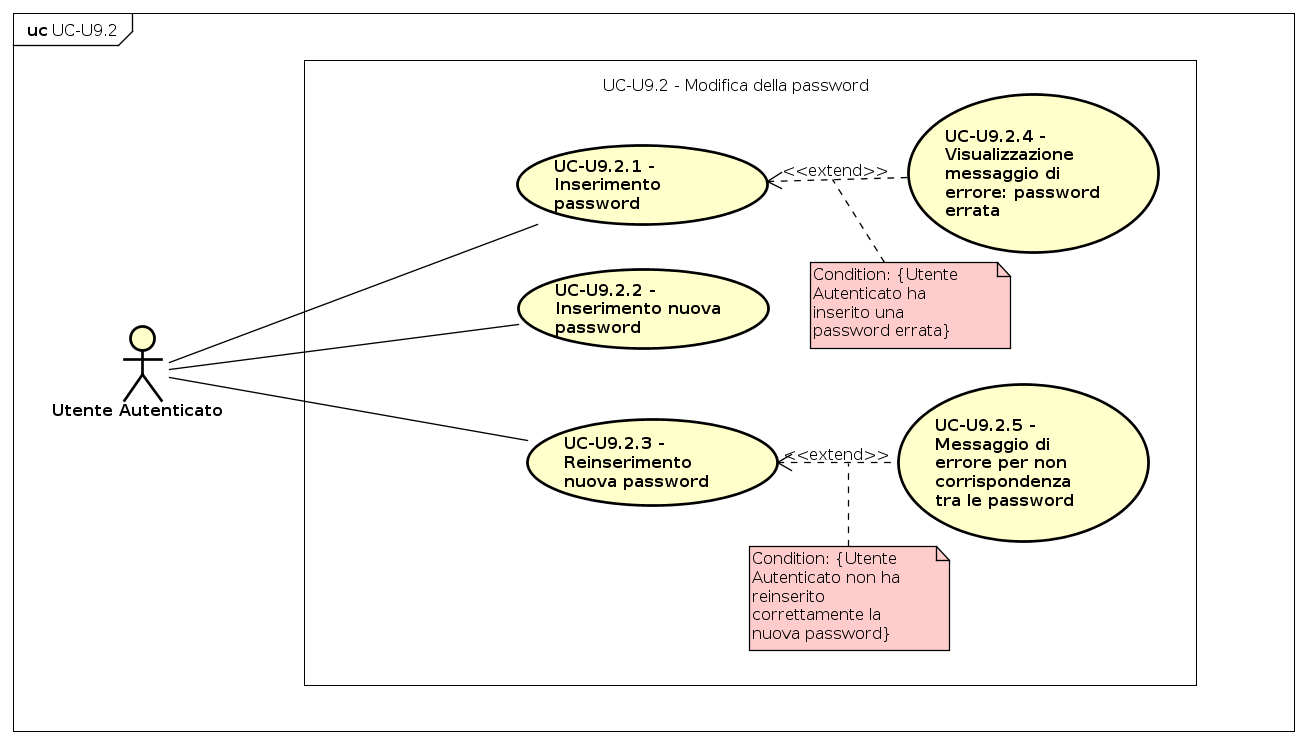
\includegraphics[width=12cm]{res/img/UCUtenti/UCUtenteA/UC-U9.2-Modifica password/UC-U9.2.png}
      \caption{UC-U9.2 - Modifica password}
      \end{center} 
    \end{figure}

    %Tabella 
    \begin{center}
      \bgroup
      \def\arraystretch{1.8}     
      \begin{longtable}{  p{3.5cm} | p{8cm} } 
        
        \hline
        \multicolumn{2}{ | c | }{ \cellcolor[gray]{0.9} \textbf{UC-U9.2 - Modifica password}} \\ 
        \hline
        
        \textbf{Attori Primari} & Utente autenticato \\ 
        \textbf{Scopo e Descrizione} & L'utente autenticato può modificare la password del proprio account. \\ 
        
        \textbf{Precondizioni}  & L'utente autenticato ha visualizzato la pagina di modifica del profilo. \\ 
        
        \textbf{Postcondizioni} & L'utente autenticato ha sostituito la password precedente con quella da lui inserita. \\ 
        \textbf{Scenario principale} & 1. L'utente autenticato inserisce la password corrente. (UC-U9.2.1)
        
2. L'utente autenticato inserisce una nuova password. (UC-U9.2.2)

3. L'utente autenticato re-inserisce la nuova password. (UC-U9.2.3) \\
        \textbf{Estensioni} & 1. L'utente autenticato visualizza un messaggio di errore dovuto all'inserimento di una password errata. (UC-U9.2.4)
        
2. L'utente autenticato visualizza un messaggio di errore causato dalla non corrispondenza tra le password inserite. (UC-U9.2.5) \\
      \end{longtable}
      \egroup
    \end{center}
    
\subsubsection{Inserimento Password}

    %Tabella 
    \begin{center}
      \bgroup
      \def\arraystretch{1.8}     
      \begin{longtable}{  p{3.5cm} | p{8cm} } 
        
        \hline
        \multicolumn{2}{ | c | }{ \cellcolor[gray]{0.9} \textbf{UC-U9.2.1 - Inserimento Password}} \\ 
        \hline
        
        \textbf{Attori Primari} & Utente autenticato \\ 
        \textbf{Scopo e Descrizione} & L'utente autenticato inserisce la propria password. \\ 
        
        \textbf{Precondizioni}  & L'utente autenticato ha visualizzato la pagina di modifica del profilo. \\ 
        
        \textbf{Postcondizioni} & L'utente autenticato ha inserito la propria password. \\ 
      \end{longtable}
      \egroup
    \end{center}
\subsubsection{Inserimento nuova password}

    %Tabella 
    \begin{center}
      \bgroup
      \def\arraystretch{1.8}     
      \begin{longtable}{  p{3.5cm} | p{8cm} } 
        
        \hline
        \multicolumn{2}{ | c | }{ \cellcolor[gray]{0.9} \textbf{UC-U9.2.2 - Inserimento nuova password}} \\ 
        \hline
        
        \textbf{Attori Primari} & Utente autenticato \\ 
        \textbf{Scopo e Descrizione} & L'utente autenticato inserisce una nuova password in sostituzione di quella precedente.  \\ 
        
        \textbf{Precondizioni}  & L'utente autenticato ha visualizzato la pagina di modifica del profilo. \\ 
        
        \textbf{Postcondizioni} & L'utente autenticato ha inserito una nuova password. \\ 
      \end{longtable}
      \egroup
    \end{center}
	
\subsubsection{Reinserimento password}

    %Tabella 
    \begin{center}
      \bgroup
      \def\arraystretch{1.8}     
      \begin{longtable}{  p{3.5cm} | p{8cm} } 
        
        \hline
        \multicolumn{2}{ | c | }{ \cellcolor[gray]{0.9} \textbf{UC-U9.2.3 - Reinserimento password}} \\ 
        \hline
        
        \textbf{Attori Primari} & Utente autenticato \\ 
        \textbf{Scopo e Descrizione} & L'utente autenticato ripete l'inserimento della nuova password. \\ 
        
        \textbf{Precondizioni}  & L'utente autenticato ha precedentemente inserito la nuova password. (UC-U9.2.2) \\ 
        
        \textbf{Postcondizioni} & L'utente autenticato ha completato la procedura di cambiamento della password. La nuova password inserita ha sostituito la password precedente. \\ 
      \end{longtable}
      \egroup
    \end{center}

\subsubsection{Visualizzazione messaggio di errore: password errata}

    %Tabella 
    \begin{center}
      \bgroup
      \def\arraystretch{1.8}     
      \begin{longtable}{  p{3.5cm} | p{8cm} } 
        
        \hline
        \multicolumn{2}{ | c | }{ \cellcolor[gray]{0.9} \textbf{UC-U9.2.4 - Visualizzazione messaggio di errore: password errata}} \\ 
        \hline
        
        \textbf{Attori Primari} & Utente autenticato \\ 
        \textbf{Scopo e Descrizione} & L'utente autenticato visualizza un messaggio di errore durante procedura di modifica del profilo dovuto all'inserimento di una password errata. \\ 
        
        \textbf{Precondizioni}  & L'utente autenticato ha inserito una password errata nella procedura di cambio della password. \\ 
        
        \textbf{Postcondizioni} & L'utente autenticato ha visualizzato il messaggio di errore. \\ 
      \end{longtable}
      \egroup
    \end{center}

\subsubsection{Messaggio di errore per non corrispondenza tra le password}

    %Tabella 
    \begin{center}
      \bgroup
      \def\arraystretch{1.8}     
      \begin{longtable}{  p{3.5cm} | p{8cm} } 
        
        \hline
        \multicolumn{2}{ | c | }{ \cellcolor[gray]{0.9} \textbf{UC-U9.2.5 - Messaggio di errore per non corrispondenza tra le password}} \\ 
        \hline
        
        \textbf{Attori Primari} & Utente autenticato \\ 
        \textbf{Scopo e Descrizione} & L'utente autenticato visualizza un messaggio di errore dovuto al reinserimento errato della nuova password (la nuova password è diversa da quella inserita la prima volta). \\ 
        
        \textbf{Precondizioni}  & L'utente autenticato non ha reinserito correttamente la nuova password. \\ 
        
        \textbf{Postcondizioni} & L'utente autenticato ha visualizzato il messaggio di errore. \\ 
      \end{longtable}
      \egroup
    \end{center}
\subsubsection{Rimozione profilo}

    %Tabella 
    \begin{center}
      \bgroup
      \def\arraystretch{1.8}     
      \begin{longtable}{  p{3.5cm} | p{8cm} } 
        
        \hline
        \multicolumn{2}{ | c | }{ \cellcolor[gray]{0.9} \textbf{UC-U9.3 - Rimozione profilo}} \\ 
        \hline
        
        \textbf{Attori Primari} & Utente autenticato \\ 
        \textbf{Scopo e Descrizione} & L'utente autenticato decide di rimuovere il suo profilo. \\ 
        
        \textbf{Precondizioni}  & L'utente autenticato ha acconsentito con la continuazione della procedura. \\ 
        
        \textbf{Postcondizioni} & L'utente autenticato visualizza un messaggio di avvenuta cancellazione e le sue credenziali vengono eliminate da MaaS. \\ 
      \end{longtable}
      \egroup
    \end{center}

\subsubsection{Procedura rimozione \glossaryItem{Company}}

%future code for UML
    \begin{figure}[H]
      \begin{center}
        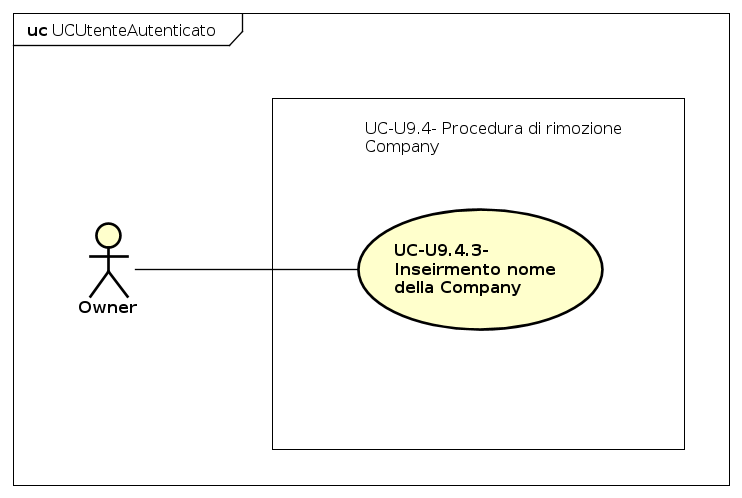
\includegraphics[width=12cm]{res/img/UCUtenti/UCUtenteA/UC-U9.4-Procedura di rimozione Company/UC-U9.4.png}
      \caption{UC-U9.4 - Procedura Rimozione}
      \end{center} 
    \end{figure}
    

    %Tabella 
    \begin{center}
      \bgroup
      \def\arraystretch{1.8}     
      \begin{longtable}{  p{3.5cm} | p{8cm} } 
        
        \hline
        \multicolumn{2}{ | c | }{ \cellcolor[gray]{0.9} \textbf{UC-U9.4 - Procedura rimozione \glossaryItem{Company}}} \\ 
        \hline
        \textbf{Attori Primari} & \glossaryItem{Owner} \\ 
        \textbf{Scopo e Descrizione} & L'\glossaryItem{Owner} decide di rimuovere la \glossaryItem{Company} con tutte le sue informazioni e i suoi utenti. \\ 
        
        \textbf{Precondizioni}  & L'\glossaryItem{Owner} inizia la procedura di cancellazione della \glossaryItem{Company} da \glossaryItem{MaaS}. \\ 
        
        \textbf{Postcondizioni} & L'\glossaryItem{Owner} ha rimosso la \glossaryItem{Company} da \glossaryItem{MaaS}. \\

        \textbf{Scenario principale} & 1. L'utente autenticato inserisce il nome della \glossaryItem{Company} corrente. (UC-U9.4.2) \\

        \textbf{Estensioni} & 1. L'utente autenticato visualizza un messaggio di errore dovuto all'inserimento del nome della \glossaryItem{Company} errata. (UC-U9.4.1)
        
      \end{longtable}
      \egroup
    \end{center}


\subsubsection{Visualizzazione messaggio d'errore}

    %Tabella 
    \begin{center}
      \bgroup
      \def\arraystretch{1.8}     
      \begin{longtable}{  p{3.5cm} | p{8cm} } 
        
        \hline
        \multicolumn{2}{ | c | }{ \cellcolor[gray]{0.9} \textbf{UC-U9.4.1 - Visualizzazione messaggio d'errore}} \\ 
        \hline
        
        \textbf{Attori Primari} & \glossaryItem{Owner} \\ 
        \textbf{Scopo e Descrizione} & L'\glossaryItem{Owner} riceve un messaggio d'errore dopo aver inserito il nome errato della \glossaryItem{Company}. \\ 
        
        \textbf{Precondizioni}  & L'\glossaryItem{Owner} non inserisce correttamente il nome della \glossaryItem{Company}. \\ 
        
        \textbf{Postcondizioni} & L'\glossaryItem{Owner} ha visualizzato il messaggio di errore. \\ 
      \end{longtable}
      \egroup
    \end{center}
    
    
\subsubsection{Rimozione \glossaryItem{Company}}

    %Tabella 
    \begin{center}
      \bgroup
      \def\arraystretch{1.8}     
      \begin{longtable}{  p{3.5cm} | p{8cm} } 
        
        \hline
        \multicolumn{2}{ | c | }{ \cellcolor[gray]{0.9} \textbf{UC-U9.4.2 - Rimozione \glossaryItem{Company}}} \\ 
        \hline
        %1) Revise the location of this use case in the whole document
        %2) This is a destructive operation, you must provide a better thought workflow
        \textbf{Attori Primari} & \glossaryItem{Owner} \\ 
        \textbf{Scopo e Descrizione} & L'\glossaryItem{Owner} decide di rimuovere la \glossaryItem{Company} con tutte le sue informazioni e i suoi utenti e si appresta a inserire il nome della \glossaryItem{Company}. \\ 
        
        \textbf{Precondizioni}  & L'\glossaryItem{Owner} ha acconsentito alla continuazione della procedura. \\ 
        
        \textbf{Postcondizioni} & L'\glossaryItem{Owner} visualizza un messaggio di avvenuto inserimento dei dati. \\ 
      \end{longtable}
      \egroup
    \end{center}

    
\subsubsection{Operazioni sulle specifiche DSL}

        \begin{figure}[H]
          \begin{center}
            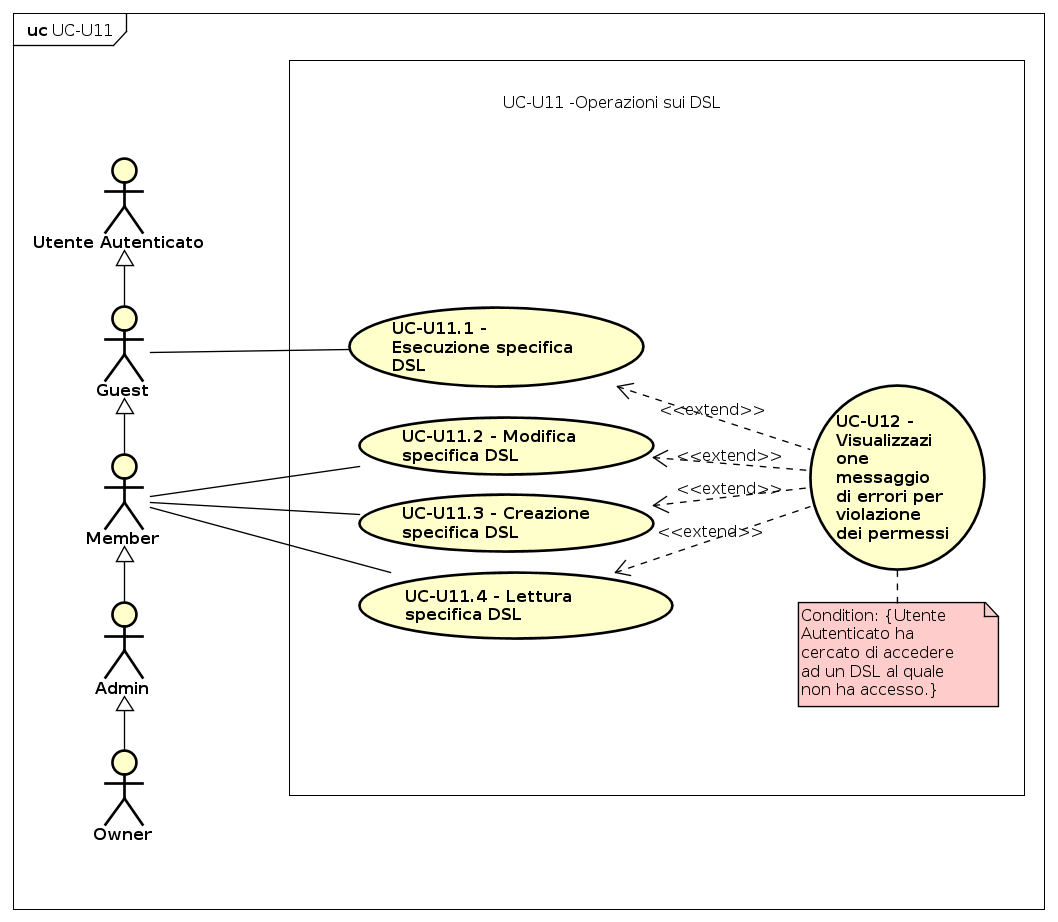
\includegraphics[width=12cm]{res/img/UCUtenti/UCUtenteA/UC-U11-Operazioni DSL/UC-U11.png}
          \caption{UC-U11 - Operazioni sulle specifiche DSL}
          \end{center} 
        \end{figure}
        
        %Tabella 
        %1) The professor says: insert only the actors which take part in one (at least) of the diagram's use cases
        %2) The term 'DSL' is not used properly
        \begin{center}
          \bgroup
          \def\arraystretch{1.8}     
          \begin{longtable}{  p{3.5cm} | p{8cm} } 
            
            \hline
            \multicolumn{2}{ | c | }{ \cellcolor[gray]{0.9} \textbf{UC-U11 - Operazioni sulle specifiche DSL}} \\ 
            \hline
            
            \textbf{Attori Primari} & Utente Autenticato, Ospite e Membro \\ 
            \textbf{Scopo e Descrizione} & L’utente visualizza la pagina per apportare modifiche sulle DSL. Può decidere di: eseguire, modificare, creare e leggere una specifica DSL.\\
            
            \textbf{Precondizioni}  & L’applicazione MaaS è funzionante e pronta all'uso. Gli utenti possono accedere alla propria pagina \glossaryItem{Dashboard}. \\ 
            
            \textbf{Postcondizioni} & Le (eventuali) modifiche sono state apportate. \\ 
            \textbf{Scenario principale} & 1. L'Ospite e il Membro possono eseguire una specifica DSL (UC-U11.1)  
            
            2. Il Membro pu\'o modificare una specifica DSL (UC-U11.2)
            
            3. Il Membro pu\'o creare una specifica DSL (UC-U11.3)
            
            4. Il Membro pu\'o leggere una specifica DSL (UC-U11.4)\\

            \textbf{Estensioni} & 1. L'utente visualizza un messaggio di errore in quanto non ha i permessi per operare sulla specifica DSL (UC-U12)  \\
          \end{longtable}
          \egroup
        \end{center}
\subsubsection{Esecuzione specifica DSL}
                %Tabella 
                \begin{center}
                  \bgroup
                  \def\arraystretch{1.8}     
                  \begin{longtable}{  p{3.5cm} | p{8cm} } 
                    
                    \hline
                    \multicolumn{2}{ | c | }{ \cellcolor[gray]{0.9} \textbf{UC-U11.1 - Esecuzione specifica DSL}} \\ 
                    \hline
                    
                    \textbf{Attori Primari} & Utente Autenticato, Ospite e Membro \\ 
                    \textbf{Scopo e Descrizione} & L'Utente Autenticato, Ospite e Membro eseguono una specifica DSL\\ 
                    
                    \textbf{Precondizioni}  & L’applicazione è funzionante e pronta all'uso. Gli utenti possono accedere alla propria pagina \glossaryItem{Dashboard}.\\ 
                    
                    \textbf{Postcondizioni} & L'utente visualizza il risultato della specifica DSL \\ 
                    \textbf{Scenario principale} & Nessuno\\
                    \textbf{Estensioni} & 1. L'utente visualizza un messaggio di errore in quanto non ha i permessi per operare sulla specifica DSL (UC-U12)  \\
                  \end{longtable}
                  \egroup
                \end{center}
\subsubsection{Modifica specifica DSL}
                %Tabella 
                \begin{center}
                  \bgroup
                  \def\arraystretch{1.8}     
                  \begin{longtable}{  p{3.5cm} | p{8cm} } 
                    
                    \hline
                    \multicolumn{2}{ | c | }{ \cellcolor[gray]{0.9} \textbf{UC-U11.2 - Modifica specifica DSL}} \\ 
                    \hline

                    \textbf{Attori Primari} & Membro  \\ 
                    \textbf{Scopo e Descrizione} & Il Membro modifica una specifica DSL tramite l'editor\\ 

                    
                    \textbf{Precondizioni}  & L’applicazione è funzionante e pronta all'uso. Gli utenti possono accedere alla propria \glossaryItem{Dashboard}. \\ 
                    
                    \textbf{Postcondizioni} & L'utente modifica la specifica DSL \\ 
                    \textbf{Estensioni} & 1. L'utente visualizza un messaggio di errore in quanto non ha i permessi per operare sulla specifica DSL (UC-U12)  \\
                  \end{longtable}
                  \egroup
                \end{center}
\subsubsection{Creazione specifica DSL}
                %Tabella 
                \begin{center}
                  \bgroup
                  \def\arraystretch{1.8}     
                  \begin{longtable}{  p{3.5cm} | p{8cm} } 
                    
                    \hline
                    \multicolumn{2}{ | c | }{ \cellcolor[gray]{0.9} \textbf{UC-U11.3 - Creazione specifica DSL}} \\ 
                    \hline
                    

                    \textbf{Attori Primari} & Membro  \\ 
                    \textbf{Scopo e Descrizione} & Il Membro crea una specifica DSL tramite l'editor\\ 
                    
                    \textbf{Precondizioni}  & L’applicazione è funzionante e pronta all'uso. Gli utenti possono accedere alla propria pagina \glossaryItem{Dashboard}.\\ 
                    
                    \textbf{Postcondizioni} & L'utente aggiunge la specifica DSL a MaaS \\ 
                    \textbf{Estensioni} & 1. L'utente visualizza un messaggio di errore in quanto non ha i permessi per operare sulla specifica DSL (UC-U12)  \\
                  \end{longtable}
                  \egroup
                \end{center}
\subsubsection{Lettura specifica DSL}
                %Tabella 
                \begin{center}
                  \bgroup
                  \def\arraystretch{1.8}     
                  \begin{longtable}{  p{3.5cm} | p{8cm} } 
                    
                    \hline
                    \multicolumn{2}{ | c | }{ \cellcolor[gray]{0.9} \textbf{UC-U11.4 - Lettura specifica DSL}} \\ 
                    \hline
                    
                    \textbf{Attori Primari} & Membro  \\ 
                    \textbf{Scopo e Descrizione} & Il Membro legge una specifica DSL\\ 
                    
                    \textbf{Precondizioni}  & L’applicazione è funzionante e pronta all'uso. Gli utenti possono accedere alla propria pagina \glossaryItem{Dashboard}.\\ 
                    
                    \textbf{Postcondizioni} & L'utente legge la specifica DSL \\ 
                    \textbf{Estensioni} & 1. L'utente visualizza un messaggio di errore in quanto non ha i permessi per operare sulla specifica DSL (UC-U12)  \\
                  \end{longtable}
                  \egroup
                \end{center}
                
                
\subsubsection{Visualizzazione di messaggio di errore per violazione dei permessi}
      
        %Tabella 
        \begin{center}
          \bgroup
          \def\arraystretch{1.8}     
          \begin{longtable}{  p{3.5cm} | p{8cm} } 
            
            \hline
            \multicolumn{2}{ | c | }{ \cellcolor[gray]{0.9} \textbf{UC-U12 - Visualizzazione di messaggio di errore per violazione dei permessi}} \\ 
            \hline
            
            \textbf{Attori Primari} & Utente autenticato \\ 
            \textbf{Scopo e Descrizione} & L’utente autenticato visualizza un messaggio di errore nel tentativo di eseguire un'operazione su una specifica DSL.\\ 
            
            \textbf{Precondizioni}  & L'utente autenticato ha eseguito un'operazione su una specifica DSL per la quale non dispone dei permessi. \\ 
            
            \textbf{Postcondizioni} & L'utente autenticato ha visualizzato il messaggio di errore. \\ 
          \end{longtable}
          \egroup
        \end{center}
\subsubsection{Operazioni sugli Utenti}

        \begin{figure}[H]
          \begin{center}
            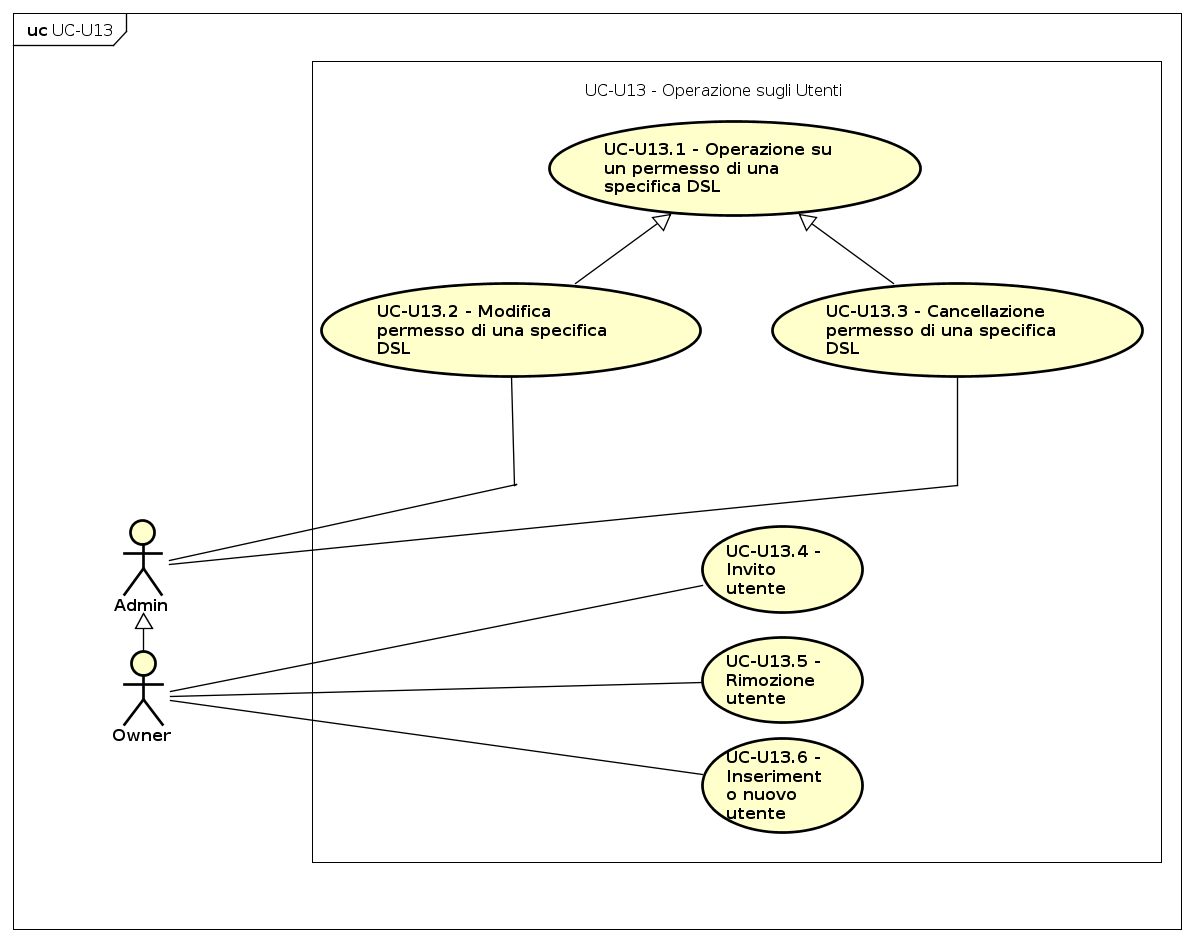
\includegraphics[width=12cm]{res/img/UCUtenti/UCUtenteA/UC-U13-Operazioni sugli Utenti/UC-U13.png}
          \caption{UC-U13 - Operazioni sugli utenti}
          \end{center} 
        \end{figure}
        
        %Tabella 
        \begin{center}
          \bgroup
          \def\arraystretch{1.8}     
          \begin{longtable}{  p{3.5cm} | p{8cm} } 
            
            \hline
            \multicolumn{2}{ | c | }{ \cellcolor[gray]{0.9} \textbf{UC-U13 - Operazioni sugli utenti}} \\ 
            \hline
            
            \textbf{Attori Primari} & Admin, \glossaryItem{Owner} \\ 
            \textbf{Scopo e Descrizione} & L'Admin e l'\glossaryItem{Owner} visualizzano la pagina per apportare modifiche sugli utenti. Possono decidere di: operare su una specifica DSL accedendo all'editor oppure inserire, rimuovere, invitare un nuovo utente.\\ 
           
            \textbf{Precondizioni}  & L'\glossaryItem{Owner} e l'Admin dispongono dei permessi per invitare/rimuovere/inserire nuovi utenti nella \glossaryItem{Company} di appartenenza.\\

              \textbf{Postcondizioni} & Le (eventuali) modifiche sono state apportate. \\ 
            \textbf{Scenario principale} & 1. L'Admin e l'\glossaryItem{Owner} possono eseguire operazioni su una specifica DSL (UC-U13.1)  
            
            2. L'\glossaryItem{Owner} può invitare un nuovo utente (UC-U13.4)
            
            3. L'\glossaryItem{Owner} può rimuovere un utente (UC-U13.5)
            
            4. L'\glossaryItem{Owner} può aggiungere un nuovo utente (UC-U13.6)\\
          \end{longtable}
          \egroup
        \end{center}
\subsubsection{Operazione su un permesso di una specifica DSL}
                %Tabella 
                \begin{center}
                  \bgroup
                  \def\arraystretch{1.8}     
                  \begin{longtable}{  p{3.5cm} | p{8cm} } 
                    
                    \hline
                    \multicolumn{2}{ | c | }{ \cellcolor[gray]{0.9} \textbf{UC-U13.1 - Operazione su un permesso di una specifica DSL}} \\ 
                    \hline
                    
                    \textbf{Attori Primari} & Amministratore, \glossaryItem{Owner} \\ 
                    \textbf{Scopo e Descrizione} & L'amministratore o l'\glossaryItem{Owner} decidono di operare su una specifica DSL\\ 
                    
                    \textbf{Precondizioni}  & La specifica DSL selezionata è già stata creata in precedenza. \\ 
                    
                    \textbf{Postcondizioni} & L'operazione sulla specifica DSL è apportata. \\ 
                  \end{longtable}
                  \egroup
                \end{center}
                
                
                
\subsubsection{Modifica permesso di una specifica DSL}
                %Tabella 
                \begin{center}
                  \bgroup
                  \def\arraystretch{1.8}     
                  \begin{longtable}{  p{3.5cm} | p{8cm} } 
                    
                    \hline
                    \multicolumn{2}{ | c | }{ \cellcolor[gray]{0.9} \textbf{UC-U13.2 - Modifica permesso di una specifica DSL}} \\ 
                    \hline
                    
                    \textbf{Attori Primari} & Amministratore, \textit{Owner} \\ 
                    \textbf{Scopo e Descrizione} & L'amministratore o l'\textit{Owner} decidono di modificare il permesso di una specifica DSL\\ 
                    
                    \textbf{Precondizioni}  & La specifica DSL selezionata è già stata creata in precedenza. \\ 
                    
                    \textbf{Postcondizioni} & La modifica sui permessi di una specifica DSL è apportata. \\ 
                  \end{longtable}
                  \egroup
                \end{center}
                
                
                
\subsubsection{Cancellazione permesso di una specifica DSL}
                %Tabella 
                \begin{center}
                  \bgroup
                  \def\arraystretch{1.8}     
                  \begin{longtable}{  p{3.5cm} | p{8cm} } 
                    
                    \hline
                    \multicolumn{2}{ | c | }{ \cellcolor[gray]{0.9} \textbf{UC-U13.3 - Cancellazione permesso di una specifica DSL}} \\ 
                    \hline
                    
                    \textbf{Attori Primari} & Amministratore, \textit{Owner} \\ 
                    \textbf{Scopo e Descrizione} & L'amministratore o l'\textit{Owner} decidono di cancellare un permesso su una specifica DSL\\ 
                    
                    \textbf{Precondizioni}  & La specifica DSL selezionata è già stata creata in precedenza. \\ 
                    
                    \textbf{Postcondizioni} & La cancellazione del permesso sulla specifica DSL è apportata. \\ 
                  \end{longtable}
                  \egroup
                \end{center}
\subsubsection{Invito utente}
                %Tabella 
                \begin{center}
                  \bgroup
                  \def\arraystretch{1.8}     
                  \begin{longtable}{  p{3.5cm} | p{8cm} } 
                    
                    \hline
                    \multicolumn{2}{ | c | }{ \cellcolor[gray]{0.9} \textbf{UC-U13.4 - Invito utente}} \\ 
                    \hline
                    
                    \textbf{Attori Primari} & \textit{Owner} \\ 
                    \textbf{Scopo e Descrizione} & L'\textit{Owner} inserisce l'indirizzo email dell'utente che vuole invitare\\ 
                    
                    \textbf{Precondizioni}  & Nessuna. \\     %%TODO: non-sense
                    
                    \textbf{Postcondizioni} & L'utente è stato invitato. \\ 
                  \end{longtable}
                  \egroup
                \end{center}
\subsubsection{Rimozione utente}
                %Tabella 
                \begin{center}
                  \bgroup
                  \def\arraystretch{1.8}     
                  \begin{longtable}{  p{3.5cm} | p{8cm} } 
                    
                    \hline
                    \multicolumn{2}{ | c | }{ \cellcolor[gray]{0.9} \textbf{UC-U13.5 - Rimozione utente}} \\ 
                    \hline
                    
                    \textbf{Attori Primari} & \textit{Owner} \\ 
                    \textbf{Scopo e Descrizione} & L'\textit{Owner} inserisce l'indirizzo email dell'utente che vuole rimuovere\\ 
                    
                    \textbf{Precondizioni}  & L'indirizzo email utente è presente in MaaS. \\ 
                    
                    \textbf{Postcondizioni} & L'utente è stato rimosso. \\ 
                  \end{longtable}
                  \egroup
                \end{center}
                
\subsubsection{Inserimento nuovo utente}
                %Tabella 
                \begin{center}
                  \bgroup
                  \def\arraystretch{1.8}     
                  \begin{longtable}{  p{3.5cm} | p{8cm} } 
                    
                    \hline
                    \multicolumn{2}{ | c | }{ \cellcolor[gray]{0.9} \textbf{UC-U13.6 - Inserimento nuovo utente}} \\ 
                    \hline
                    
                    \textbf{Attori Primari} & \textit{Owner} \\ 
                    \textbf{Scopo e Descrizione} & L'\textit{Owner} inserisce un nuovo utente all'applicazione.\\ 
                    
                    \textbf{Precondizioni}  & Nessuna \\ 
                    
                    \textbf{Postcondizioni} & Un nuovo utente \`e stato aggiunto a \glossaryItem{MaaS}. \\ 
                  \end{longtable}
                  \egroup
                \end{center}

\subsubsection{Visualizzazione di messaggio di errore per indirizzo email già presente}

    %Tabella 
    \begin{center}
      \bgroup
      \def\arraystretch{1.8}     
      \begin{longtable}{  p{3.5cm} | p{8cm} } 
        
        \hline
        \multicolumn{2}{ | c | }{ \cellcolor[gray]{0.9} \textbf{UC-U13.6.2 - Visualizzazione di messaggio di errore per indirizzo email già presente}} \\ 
        \hline
        
        \textbf{Attori Primari} & Utente autenticato \\ 
        \textbf{Scopo e Descrizione} & L'utente autenticato visualizza un messaggio di errore durante la procedura di modifica del profilo causato dall'inserimento di un indirizzo email già presente nel sistema. \\ 
        
        \textbf{Precondizioni}  & L'utente autenticato ha inserito un indirizzo email già presente nel sistema. \\ 
        
        \textbf{Postcondizioni} & L'utente autenticato ha visualizzato il messaggio di errore. \\ 
      \end{longtable}
      \egroup
    \end{center}
                
                
\subsubsection{Visualizzazione di messaggio di errore per violazione dei permessi}
      
        %Tabella 
        \begin{center}
          \bgroup
          \def\arraystretch{1.8}     
          \begin{longtable}{  p{3.5cm} | p{8cm} } 
            
            \hline
            \multicolumn{2}{ | c | }{ \cellcolor[gray]{0.9} \textbf{UC-U14 - Visualizzazione di messaggio di errore per violazione dei permessi}} \\ 
            \hline
            
            \textbf{Attori Primari} & Utente autenticato \\ 
            \textbf{Scopo e Descrizione} & L’utente autenticato visualizza un messaggio di errore nel tentativo di eseguire un'operazione su un utente.\\ 
            
            \textbf{Precondizioni}  & L'utente autenticato ha eseguito un'operazione su un utente di cui non dispone i permessi. \\ 
            
            \textbf{Postcondizioni} & L'utente autenticato ha visualizzato il messaggio di errore. \\ 
          \end{longtable}
          \egroup
        \end{center}
\subsubsection{Operazioni \glossaryItem{Dashboard}}
 

    \begin{figure}[H]
      \begin{center}
        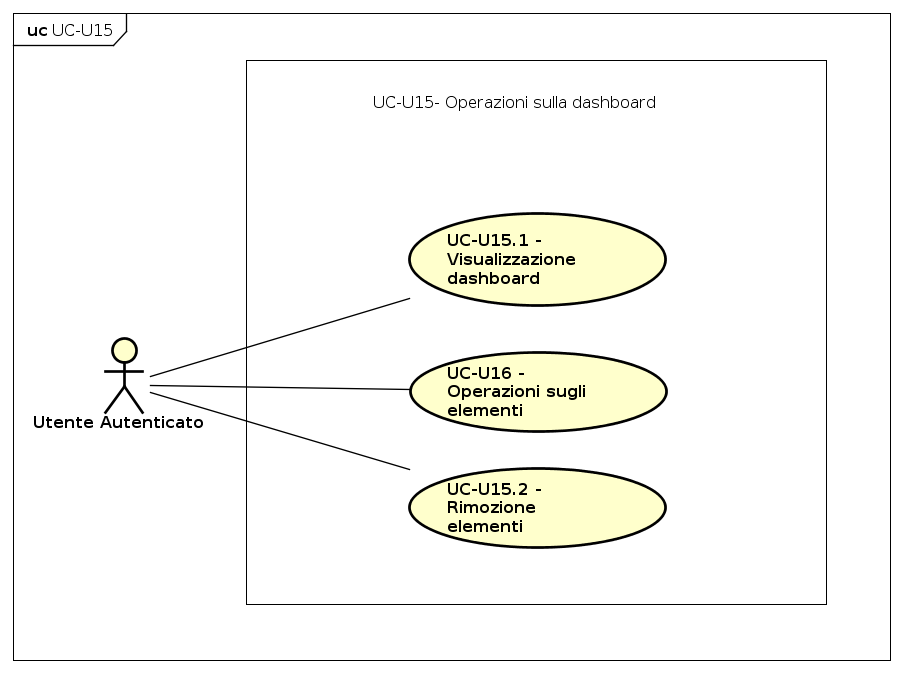
\includegraphics[width=12cm]{res/img/UCUtenti/UCUtenteA/UC-U15-Operazioni-dashboard/UC-U15.png}
      \caption{UC-U15 - Operazioni \glossaryItem{Dashboard}}
      \end{center} 
    \end{figure}

    %Tabella 
    \begin{center}
      \bgroup
      \def\arraystretch{1.8}     
      \begin{longtable}{  p{3.5cm} | p{8cm} } 
        
        \hline
        \multicolumn{2}{ | c | }{ \cellcolor[gray]{0.9} \textbf{UC-U15 - Operazioni \glossaryItem{Dashboard}}} \\ 
        \hline
        
        \textbf{Attori Primari} & Utente autenticato \\ 
        \textbf{Scopo e Descrizione} & L'utente autenticato può: visualizzare la \glossaryItem{Dashboard}, effettuare delle operazioni sulle righe della \glossaryItem{Dashboard}, rimuovere le righe della \glossaryItem{Dashboard}. \\ 
        
        \textbf{Precondizioni}  & L'utente autenticato si trova nella pagina iniziale \glossaryItem{Dashboard}. \\ 
        
        \textbf{Postcondizioni} & L'applicazione MaaS ha eseguito le operazioni richieste dall'utente. \\ 
        \textbf{Scenario principale} & 1. L'utente autenticato visualizza la \glossaryItem{Dashboard} (UC-U15.1)
        
2. L'utente autenticato effettua delle operazioni su un elemento della \glossaryItem{Dashboard} (UC-U16)

3. L'utente autenticato rimuove degli elementi dalla \glossaryItem{Dashboard} (UC-U15.2) \\
      \end{longtable}
      \egroup
    \end{center}

\subsubsection{Visualizzazione \glossaryItem{Dashboard}}

    %Tabella 
    \begin{center}
      \bgroup
      \def\arraystretch{1.8}     
      \begin{longtable}{  p{3.5cm} | p{8cm} } 
        
        \hline
        \multicolumn{2}{ | c | }{ \cellcolor[gray]{0.9} \textbf{UC-U15.1 - Visualizzazione \glossaryItem{Dashboard}}} \\ 
        \hline
        
        \textbf{Attori Primari} & Utente autenticato \\ 
        \textbf{Scopo e Descrizione} & L'utente autenticato visualizza la \glossaryItem{Dashboard}. \\ 
        
        \textbf{Precondizioni}  & L'applicazione mostra la \glossaryItem{Dashboard}. \\ 
        
        \textbf{Postcondizioni} & L'utente ha visualizzato la propria \glossaryItem{Dashboard}. \\ 
      \end{longtable}
      \egroup
    \end{center}
    
\subsubsection{Rimozione elementi \glossaryItem{Dashboard}}

    %Tabella 
    \begin{center}
      \bgroup
      \def\arraystretch{1.8}     
      \begin{longtable}{  p{3.5cm} | p{8cm} } 
        
        \hline
        \multicolumn{2}{ | c | }{ \cellcolor[gray]{0.9} \textbf{UC-U15.2 - Rimozione elementi \glossaryItem{Dashboard}}} \\ 
        \hline
        
        \textbf{Attori Primari} & Utente autenticato \\ 
        \textbf{Scopo e Descrizione} & L'utente autenticato intende eliminare degli elementi presenti nella sua \glossaryItem{Dashboard}. \\ 
        
        \textbf{Precondizioni}  & L'utente si trova nella pagina \glossaryItem{Dashboard} e seleziona l'elemento che vuole eliminare. \\ 
        
        \textbf{Postcondizioni} & Il sistema ha rimosso l'elemento. \\ 
      \end{longtable}
      \egroup
    \end{center}

\subsubsection{Operazioni sugli elementi della \glossaryItem{Dashboard}}

    \begin{figure}[H]
      \begin{center}
        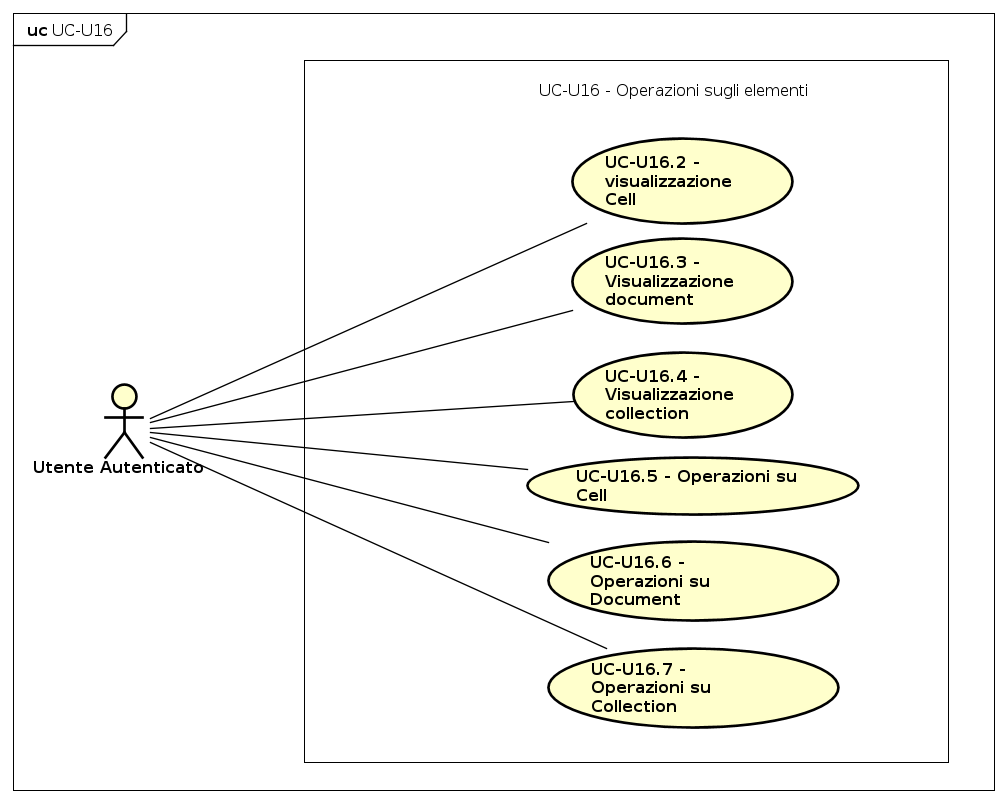
\includegraphics[width=12cm]{res/img/UCUtenti/UCUtenteA/UC-U16-Operazioni_sulle_righe/UC-U16.png}
      \caption{UC-U16 - Operazioni sugli elementi della \glossaryItem{Dashboard}}
      \end{center} 
    \end{figure}

    %Tabella 
    \begin{center}
      \bgroup
      \def\arraystretch{1.8}     
      \begin{longtable}{  p{3.5cm} | p{8cm} } 
        
        \hline
        \multicolumn{2}{ | c | }{ \cellcolor[gray]{0.9} \textbf{UC-U16 - Operazioni sugli elementi della \glossaryItem{Dashboard}}} \\ 
        \hline
        
        \textbf{Attori Primari} & Utente autenticato \\ 
        \textbf{Scopo e Descrizione} & L'utente autenticato può eseguire le seguenti azioni sugli elementi della \glossaryItem{Dashboard}: visualizzare un elemento (che può essere una \glossaryItem{Cell}, un \glossaryItem{Document} o una \glossaryItem{Collection}) oppure effettuare un'operazione su di esso. \\ 
        
        \textbf{Precondizioni}  & L'utente autenticato ha visualizzato la pagina iniziale \glossaryItem{Dashboard}. \\ 
        
        \textbf{Postcondizioni} & L'applicazione ha eseguito le operazioni sulle righe della \glossaryItem{Dashboard} richieste dall'utente autenticato. \\ 
        \textbf{Scenario principale} & 1. Visualizzazione element \glossaryItem{Dashboard} (UC-U16.1)
        
1.1 L'utente visualizza una \glossaryItem{Cell} (UC-U16.2)

1.2 L'utente visualizza un \glossaryItem{Document} (UC-U16.3)

1.3 L'utente visualizza una \glossaryItem{Collection} (UC-U16.4)

2. L'utente desidera effettuare un'operazione su una riga

2.1 L'utente effettua un'operazione su una \glossaryItem{Cell} (UC-U16.5)

2.2 L'utente effettua un'operazione su un \glossaryItem{Document} (UC-U16.6)

2.3 L'utente effettua un'operazione su una \glossaryItem{Collection} (UC-U16.7) \\
      \end{longtable}
      \egroup
    \end{center}
    

\subsubsection{Visualizzazione element \glossaryItem{Dashboard}}
    %Tabella 
    \begin{center}
      \bgroup
      \def\arraystretch{1.8}     
      \begin{longtable}{  p{3.5cm} | p{8cm} } 
        
        \hline
        \multicolumn{2}{ | c | }{ \cellcolor[gray]{0.9} \textbf{UC-U16.1 - Visualizzazione element \glossaryItem{Dashboard}}} \\ 
        \hline
        
        \textbf{Attori Primari} & Utente autenticato \\ 
        \textbf{Scopo e Descrizione} & L'utente autenticato può visualizzare un element dalla \glossaryItem{Dashboard} (che può essere una \glossaryItem{Cell}, un \glossaryItem{Document} o una \glossaryItem{Collection}). \\ 
        
        \textbf{Precondizioni}  & L'utente autenticato ha visualizzato la pagina \glossaryItem{Dashboard}. \\ 
        
        \textbf{Postcondizioni} & L'utente autenticato viene reindirizzato alla pagina di visione dell'element selezionato. \\ 
      \end{longtable}
      \egroup
    \end{center}

\newpage

\subsubsection{Visualizzazione \glossaryItem{Cell}}

    %Tabella 
    \begin{center}
      \bgroup
      \def\arraystretch{1.8}     
      \begin{longtable}{  p{3.5cm} | p{8cm} } 
        
        \hline
        \multicolumn{2}{ | c | }{ \cellcolor[gray]{0.9} \textbf{UC-U16.2 - Visualizzazione \glossaryItem{Cell}}} \\ 
        \hline
        
        \textbf{Attori Primari} & Utente autenticato \\ 
        \textbf{Scopo e Descrizione} & L'utente autenticato può visualizzare una \glossaryItem{Cell} selezionata nella \glossaryItem{Dashboard}. \\ 
        
        \textbf{Precondizioni}  & L'utente autenticato ha visualizzato la pagina \glossaryItem{Dashboard}. \\ 
        
        \textbf{Postcondizioni} & L'utente autenticato è stato reindirizzato nella pagina \glossaryItem{Cell} e ne ha visualizzato il contenuto. \\ 
      \end{longtable}
      \egroup
    \end{center}
    
\subsubsection{Visualizzazione \glossaryItem{Document}}

    %Tabella 
    \begin{center}
      \bgroup
      \def\arraystretch{1.8}     
      \begin{longtable}{  p{3.5cm} | p{8cm} } 
        
        \hline
        \multicolumn{2}{ | c | }{ \cellcolor[gray]{0.9} \textbf{UC-U16.3 - Visualizzazione \glossaryItem{Document}}} \\ 
        \hline
        
        \textbf{Attori Primari} & Utente autenticato \\ 
        \textbf{Scopo e Descrizione} & L'utente autenticato può visualizzare un \glossaryItem{Document} selezionato nella \glossaryItem{Dashboard}. \\ 
        
        \textbf{Precondizioni}  & L'utente autenticato ha visualizzato la pagina \glossaryItem{Dashboard}. \\ 
        
        \textbf{Postcondizioni} & L'utente autenticato è stato reindirizzato nella pagina \glossaryItem{Document} e ne ha visualizzato il contenuto. \\ 
      \end{longtable}
      \egroup
    \end{center}
    
\subsubsection{Visualizzazione \glossaryItem{Collection}}

    %Tabella 
    \begin{center}
      \bgroup
      \def\arraystretch{1.8}     
      \begin{longtable}{  p{3.5cm} | p{8cm} } 
        
        \hline
        \multicolumn{2}{ | c | }{ \cellcolor[gray]{0.9} \textbf{UC-U16.4 - Visualizzazione \glossaryItem{Collection}}} \\ 
        \hline
        
        \textbf{Attori Primari} & Utente autenticato \\ 
        \textbf{Scopo e Descrizione} & L'utente autenticato può visualizzare una \glossaryItem{Collection} selezionato nella \glossaryItem{Dashboard}. \\ 
        
        \textbf{Precondizioni}  & L'utente autenticato ha visualizzato la pagina \glossaryItem{Dashboard}. \\ 
        
        \textbf{Postcondizioni} & L'utente autenticato è stato reindirizzato nella pagina \glossaryItem{Collection} e ne ha visualizzato il contenuto. \\ 
      \end{longtable}
      \egroup
    \end{center}
    
\subsubsection{Operazioni su \glossaryItem{Cell}}
 

    \begin{figure}[H]
      \begin{center}
        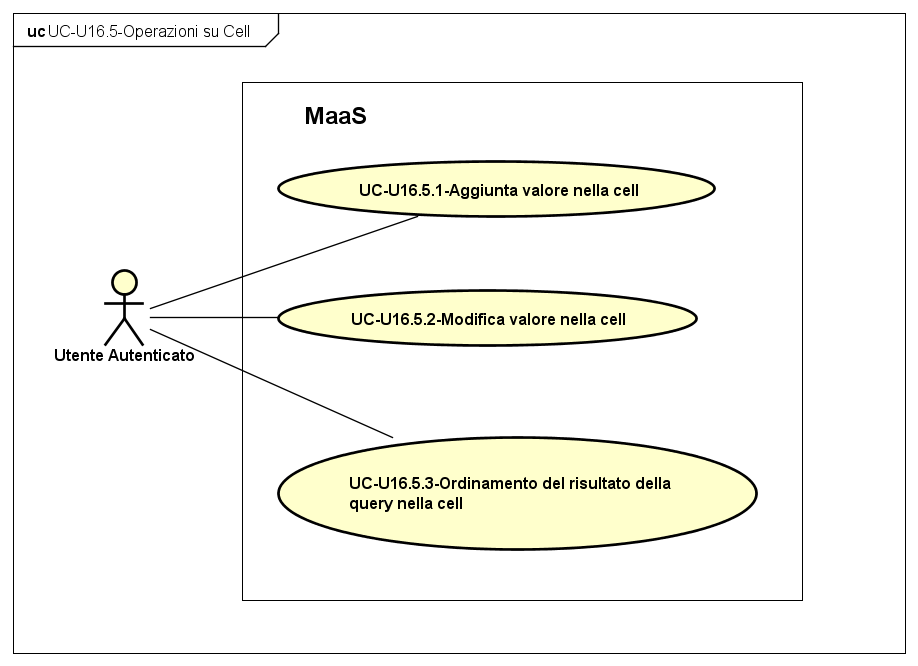
\includegraphics[width=12cm]{res/img/UCUtenti/UCUtenteA/UC-U16.5-Operazioni_su_Cell/UC-U16.5-Operazioni_su_Cell}
      \caption{UC-U16.5 - Operazioni su \glossaryItem{Cell}}
      \end{center} 
    \end{figure}

    %Tabella 
    \begin{center}
      \bgroup
      \def\arraystretch{1.8}     
      \begin{longtable}{  p{3.5cm} | p{8cm} } 
        
        \hline
        \multicolumn{2}{ | c | }{ \cellcolor[gray]{0.9} \textbf{UC-U16.5 - Operazioni su \glossaryItem{Cell}}} \\ 
        \hline
        
        \textbf{Attori Primari} & Utente autenticato \\ 
        \textbf{Scopo e Descrizione} & L'utente autenticato può eseguire le seguenti operazioni dalla pagina \glossaryItem{Cell}: può aggiungere un valore arbitrario, può modificarne uno, può ordinare il valore nella \glossaryItem{Cell} in base all'unico campo della query (scritta in un momento precedente nell'editor) che ha prodotto tale valore. \\ 
        
        \textbf{Precondizioni}  & L'utente autenticato ha visualizzato la pagina \glossaryItem{Cell}. \\ 
        
        \textbf{Postcondizioni} & L'applicazione MaaS ha eseguito le operazioni richieste dall'utente autenticato. \\ 
        \textbf{Scenario principale} & 1. L'utente autenticato aggiunge un valore arbitrario nella \glossaryItem{Cell}. (UC-U16.5.1)
        
2. L'utente autenticato modifica il valore nella \glossaryItem{Cell}. (UC-U16.5.2)

3. L'utente autenticato ordina il valore nella \glossaryItem{Cell}. (UC-U16.5.3) \\
      \end{longtable}
      \egroup
    \end{center}
	
\subsubsection{Aggiunta di un valore nella \glossaryItem{Cell}}

    %Tabella 
    \begin{center}
      \bgroup
      \def\arraystretch{1.8}     
      \begin{longtable}{  p{3.5cm} | p{8cm} } 
        
        \hline
        \multicolumn{2}{ | c | }{ \cellcolor[gray]{0.9} \textbf{UC-U16.5.1 - Aggiunta di un valore nella \glossaryItem{Cell}}} \\ 
        \hline
        
        \textbf{Attori Primari} & Utente autenticato \\ 
        \textbf{Scopo e Descrizione} & L'utente autenticato può aggiungere un valore arbitrario nella \glossaryItem{Cell}.  \\ 
        
        \textbf{Precondizioni}  & L'utente autenticato ha visualizzato la pagina \glossaryItem{Cell}.  \\ 
        
        \textbf{Postcondizioni} & L'utente autenticato ha aggiunto un valore arbitrario nella \glossaryItem{Cell}. \\ 
      \end{longtable}
      \egroup
    \end{center}
    
\subsubsection{Modifica valore \glossaryItem{Cell}}

    %Tabella 
    \begin{center}
      \bgroup
      \def\arraystretch{1.8}     
      \begin{longtable}{  p{3.5cm} | p{8cm} } 
        
        \hline
        \multicolumn{2}{ | c | }{ \cellcolor[gray]{0.9} \textbf{UC-U16.5.2 - Modifica valore \glossaryItem{Cell}}} \\ 
        \hline
        
        \textbf{Attori Primari} & Utente autenticato \\ 
        \textbf{Scopo e Descrizione} & L'utente autenticato può modificare il valore della \glossaryItem{Cell}. \\ 
        
        \textbf{Precondizioni}  & L'utente autenticato ha visualizzato la pagina \glossaryItem{Cell}. \\ 
        
        \textbf{Postcondizioni} & L'utente autenticato ha modificato il valore della \glossaryItem{Cell}. \\ 
      \end{longtable}
      \egroup
    \end{center}
\subsubsection{Ordinamento \glossaryItem{Cell}}

    %Tabella 
    \begin{center}
      \bgroup
      \def\arraystretch{1.8}     
      \begin{longtable}{  p{3.5cm} | p{8cm} } 
        
        \hline
        \multicolumn{2}{ | c | }{ \cellcolor[gray]{0.9} \textbf{UC-U16.5.3 - Ordinamento \glossaryItem{Cell}}} \\ 
        \hline
        
        \textbf{Attori Primari} & Utente autenticato \\ 
        \textbf{Scopo e Descrizione} & L'utente autenticato può ordinare il valore nella \glossaryItem{Cell} in base all'unico campo della query (scritta in un momento precedente nell'editor) che ha prodotto tale valore. \\ 
        
        \textbf{Precondizioni}  & L'utente autenticato ha visualizzato la pagina \glossaryItem{Cell}. \\ 
        
        \textbf{Postcondizioni} & L'utente autenticato ha ordinato il valore della \glossaryItem{Cell}. \\ 
      \end{longtable}
      \egroup
    \end{center}

\subsubsection{Operazioni su \glossaryItem{Document}}
 

    \begin{figure}[H]
      \begin{center}
        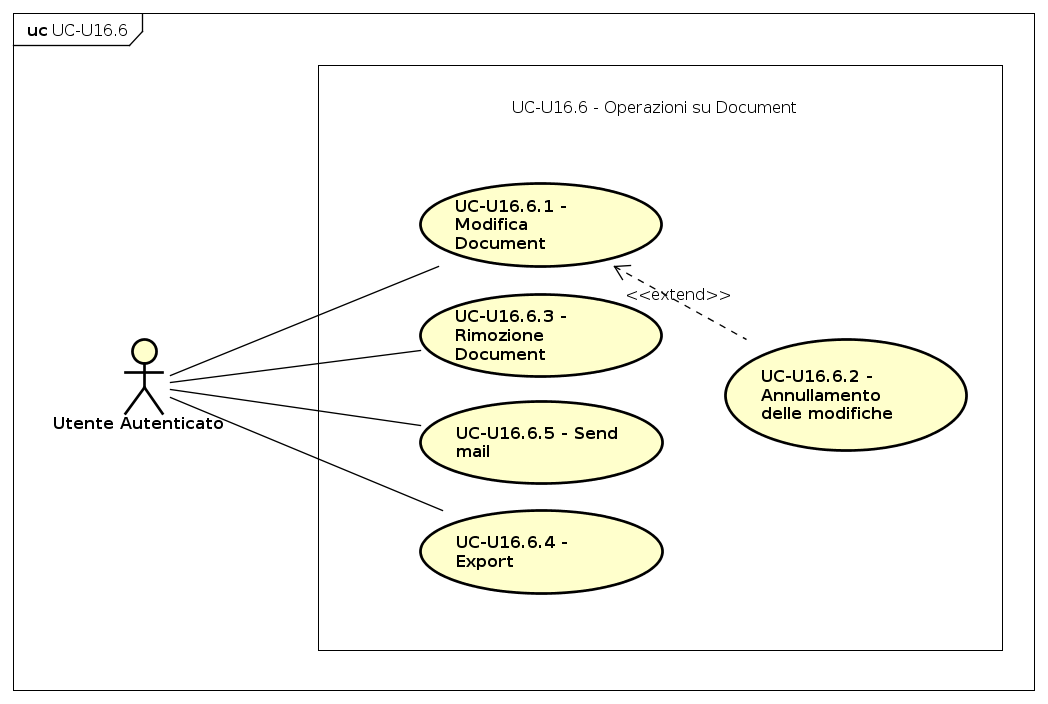
\includegraphics[width=12cm]{res/img/UCUtenti/UCUtenteA/UC-U16.6-Operazioni_su_Document/UC-U16.6}
      \caption{UC-U16.6 - Operazioni su \glossaryItem{Document}}
      \end{center} 
    \end{figure}

    %Tabella 
    \begin{center}
      \bgroup
      \def\arraystretch{1.8}     
      \begin{longtable}{  p{3.5cm} | p{8cm} } 
        
        \hline
        \multicolumn{2}{ | c | }{ \cellcolor[gray]{0.9} \textbf{UC-U16.6 - Operazioni su \glossaryItem{Document}}} \\ 
        \hline
        
        \textbf{Attori Primari} & Utente autenticato \\ 
        \textbf{Scopo e Descrizione} & L'utente autenticato può effettuare le seguenti operazioni sul \textit{Document}: modificarlo, rimuoverlo, eseguire un'operazione di `Export' o di `Send mail'. \\ 
        
        \textbf{Precondizioni}  & L'utente autenticato ha visualizzato la pagina \glossaryItem{Document}. \\ 
        
        \textbf{Postcondizioni} & L'applicazione MaaS ha eseguito le operazioni richieste dall'utente autenticato. \\ 
        \textbf{Scenario principale} & 1. L'utente autenticato modifica un \glossaryItem{Document} (UC-U16.6.1)
        
2. L'utente autenticato rimuove un \glossaryItem{Document} (UC-U16.6.3)

3. L'utente autenticato esporta il \textit{Document} in formato \textit{json} o \textit{csv} (UC-U16.6.4)

4. L'utente autenticato invia una mail a un altro utente (UC-U16.6.5)\\
        \textbf{Estensioni} & 1. L'utente desidera annullare le modifiche apportate a un \glossaryItem{Document} (UC-U16.6.2) \\
      \end{longtable}
      \egroup
    \end{center}
    
\subsubsection{Modifica \glossaryItem{Document}}

    %Tabella 
    \begin{center}
      \bgroup
      \def\arraystretch{1.8}     
      \begin{longtable}{  p{3.5cm} | p{8cm} } 
        
        \hline
        \multicolumn{2}{ | c | }{ \cellcolor[gray]{0.9} \textbf{UC-U16.6.1 - Modifica \glossaryItem{Document}}} \\ 
        \hline
        
        \textbf{Attori Primari} & Utente autenticato \\ 
        \textbf{Scopo e Descrizione} & L'utente autenticato può modificare un \glossaryItem{Document} (modifica il valore di uno dei campi visualizzati nella pagina \glossaryItem{Document} selezionata). \\ 
        
        \textbf{Precondizioni}  & L'utente autenticato ha visualizzato una pagina \glossaryItem{Document} all'interno della quale desidera apportare delle modifiche. \\ 
        
        \textbf{Postcondizioni} & L'applicazione MaaS ha apportato le modifiche richieste dall'utente al \glossaryItem{Document} selezionato. \\ 
      \end{longtable}
      \egroup
    \end{center}
    
\subsubsection{Annullamento delle modifiche di \glossaryItem{Document}}

    %Tabella 
    \begin{center}
      \bgroup
      \def\arraystretch{1.8}     
      \begin{longtable}{  p{3.5cm} | p{8cm} } 
        
        \hline
        \multicolumn{2}{ | c | }{ \cellcolor[gray]{0.9} \textbf{UC-U16.6.2 - Annullamento delle modifiche di \glossaryItem{Document}}} \\ 
        \hline
        
        \textbf{Attori Primari} & Utente autenticato \\ 
        \textbf{Scopo e Descrizione} & L'utente autenticato può annullare le modifiche precedentemente apportate al \glossaryItem{Document} selezionato. \\ 
        
        \textbf{Precondizioni}  & L'utente autenticato ha apportato delle modifiche a un \glossaryItem{Document}. \\ 
        
        \textbf{Postcondizioni} & Le modifiche apportate dall'utente autenticato al \glossaryItem{Document} selezionato sono state annullate. \\ 
      \end{longtable}
      \egroup
    \end{center}

\subsubsection{Rimozione \glossaryItem{Document}}

    %Tabella 
    \begin{center}
      \bgroup
      \def\arraystretch{1.8}     
      \begin{longtable}{  p{3.5cm} | p{8cm} } 
        
        \hline
        \multicolumn{2}{ | c | }{ \cellcolor[gray]{0.9} \textbf{UC-U16.6.3 - Rimozione \glossaryItem{Document}}} \\ 
        \hline
        
        \textbf{Attori Primari} & Utente autenticato \\ 
        \textbf{Scopo e Descrizione} & L'utente autenticato può rimuovere un \glossaryItem{Document} dalla \glossaryItem{Dashboard}. \\ 
        
        \textbf{Precondizioni}  & L'utente autenticato ha visualizzato la pagina \glossaryItem{Document} da rimuovere. \\ 
        
        \textbf{Postcondizioni} & La pagina \glossaryItem{Document} selezionata è stata rimossa. \\ 
      \end{longtable}
      \egroup
    \end{center}
    
\subsubsection{Export di un \glossaryItem{Document}}

    %Tabella 
    \begin{center}
      \bgroup
      \def\arraystretch{1.8}     
      \begin{longtable}{  p{3.5cm} | p{8cm} } 
        
        \hline
        \multicolumn{2}{ | c | }{ \cellcolor[gray]{0.9} \textbf{UC-U16.6.4 - Export di un \glossaryItem{Document}}} \\ 
        \hline
        
        \textbf{Attori Primari} & Utente autenticato \\ 
        \textbf{Scopo e Descrizione} & L'utente autenticato può esportare il \textit{Document} corrente in formato
        \textit{json} o \textit{csv}. \\ 
        
        \textbf{Precondizioni}  & L'utente autenticato ha visualizzato la pagina del \glossaryItem{Document} su cui effettuare le operazioni di `Export' o di `Send email'. \\ 
        
        \textbf{Postcondizioni} & L'applicazione MaaS ha eseguito la richiesta dell'utente. \\ 
      \end{longtable}
      \egroup
    \end{center}
    
\subsubsection{Send Mail da un \glossaryItem{Document}}

    %Tabella 
    \begin{center}
      \bgroup
      \def\arraystretch{1.8}     
      \begin{longtable}{  p{3.5cm} | p{8cm} } 
        
        \hline
        \multicolumn{2}{ | c | }{ \cellcolor[gray]{0.9} \textbf{UC-U16.6.5 - Send Mail da un \glossaryItem{Document}}} \\ 
        \hline
        
        \textbf{Attori Primari} & Utente autenticato \\ 
        \textbf{Scopo e Descrizione} & L'utente autenticato può inviare una mail contenente il \glossaryItem{Document} a un altro utente. \\ 
        
        \textbf{Precondizioni}  & L'utente autenticato ha visualizzato la pagina \glossaryItem{Document} su cui effettuare l'operazione di `Send mail`. \\ 
        
        \textbf{Postcondizioni} & L'applicazione ha inviato la mail con il \glossaryItem{Document} al destinatario segnalato dall'utente. \\ 
      \end{longtable}
      \egroup
    \end{center}


    
\subsubsection{Operazioni su \glossaryItem{Collection}}
 

    \begin{figure}[H]
      \begin{center}
        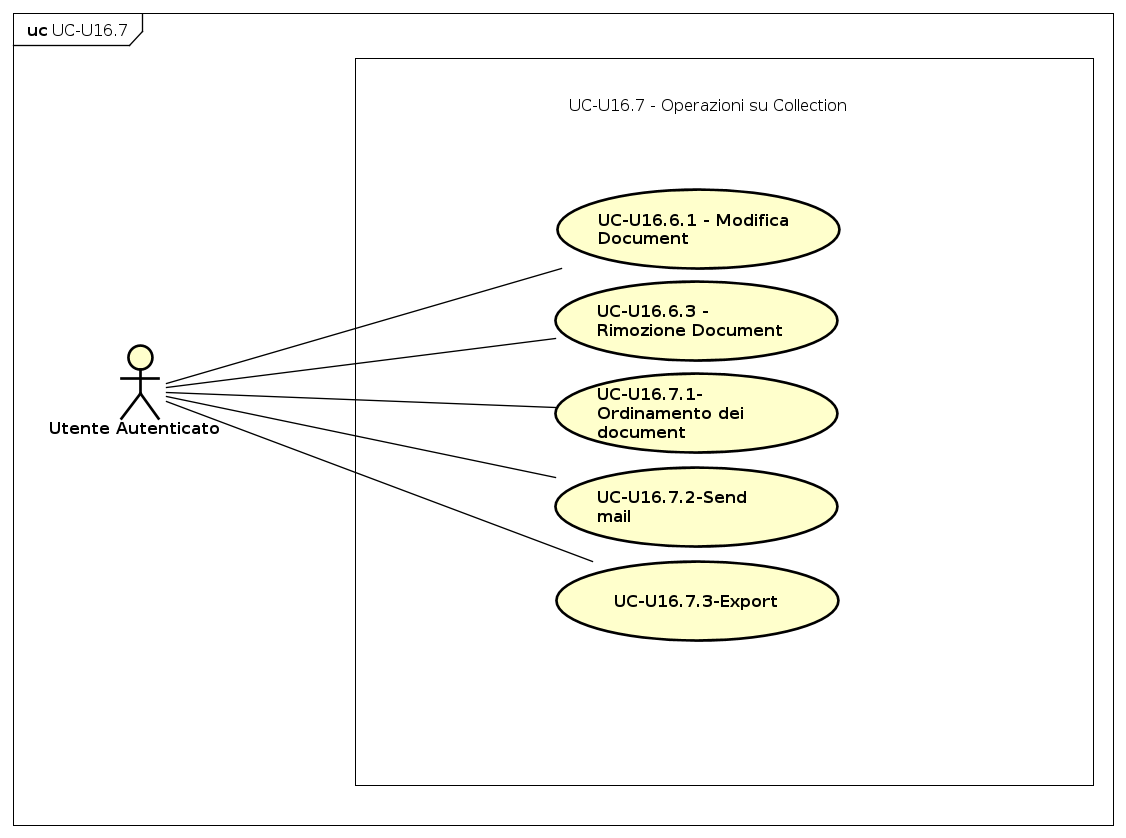
\includegraphics[width=12cm]{res/img/UCUtenti/UCUtenteA/UC-U16.7-Operazioni_su_Collection/UC-U16.7.png}
      \caption{UC-U16.7 - Operazioni su \glossaryItem{Collection}}
      \end{center} 
    \end{figure}

    %Tabella 
    \begin{center}
      \bgroup
      \def\arraystretch{1.8}     
      \begin{longtable}{  p{3.5cm} | p{8cm} } 
        
        \hline
        \multicolumn{2}{ | c | }{ \cellcolor[gray]{0.9} \textbf{UC-U16.7 - Operazioni su \glossaryItem{Collection}}} \\ 
        \hline
        
        \textbf{Attori Primari} & Utente autenticato \\ 
        \textbf{Scopo e Descrizione} & L'utente autenticato può eseguire una delle seguenti operazioni su un pagina \glossaryItem{Collection}: modificare un \glossaryItem{Document}, filtrare i \glossaryItem{Document}, selezionare e visualizzare un sottoinsieme di attributi di un sottoinsieme di \glossaryItem{Document}, rimuovere un \glossaryItem{Document}, eseguire un'azione di default (Export o Send Mail), o un'azione personalizzata. \\ 
        
        \textbf{Precondizioni}  & L'utente autenticato ha visualizzato la pagina \glossaryItem{Collection}. \\ 
        
        \textbf{Postcondizioni} & L'applicazione MaaS ha eseguito le operazioni richieste dall'utente autenticato. \\ 
        \textbf{Scenario principale} & 1. L'utente autenticato può modificare un \glossaryItem{Document} (UC-U16.6.1)

2. L'utente autenticato può ordinare i Documents. (UC-U16.7.1)

3. L'utente autenticato può rimuovere un \glossaryItem{Document}. (UC-U16.6.3)

4. L'utente autenticato può eseguire l'azione di `send mail`. (UC-U16.7.2)

5. L'utente autenticato può eseguire l'azione di `export` su un insieme di \glossaryItem{Document}. (UC-U16.7.3) \\

      \end{longtable}
      \egroup
    \end{center}
    
\subsubsection{Ordina \glossaryItem{Document}}

    %Tabella 
    \begin{center}
      \bgroup
      \def\arraystretch{1.8}     
      \begin{longtable}{  p{3.5cm} | p{8cm} } 
        
        \hline
        \multicolumn{2}{ | c | }{ \cellcolor[gray]{0.9} \textbf{UC-U16.7.1 - Ordina \glossaryItem{Document}}} \\ 
        \hline
        
        \textbf{Attori Primari} & Utente autenticato \\ 
        \textbf{Scopo e Descrizione} & L'utente autenticato può decidere di ordinare i \glossaryItem{Document} della \glossaryItem{Collection} in base a uno dei loro attributi. \\ 
        
        \textbf{Precondizioni}  & L'utente autenticato ha visualizzato la pagina \glossaryItem{Collection}. \\ 
        
        \textbf{Postcondizioni} & L'applicazione ha ordinato i \glossaryItem{Document} secondo l'ordine indicato dall'utente. \\ 
      \end{longtable}
      \egroup
    \end{center}
    
      

    
\subsubsection{Send mail da una \glossaryItem{Collection}}

    %Tabella 
    \begin{center}
      \bgroup
      \def\arraystretch{1.8}     
      \begin{longtable}{  p{3.5cm} | p{8cm} } 
        
        \hline
        \multicolumn{2}{ | c | }{ \cellcolor[gray]{0.9} \textbf{UC-U16.7.2 - Send mail da una \glossaryItem{Collection}}} \\ 
        \hline
        
        \textbf{Attori Primari} & Utente autenticato \\ 
        \textbf{Scopo e Descrizione} & L'utente autenticato può inviare una email contenente i Documents selezionati a un altro utente. \\ 
        
        \textbf{Precondizioni}  & L'utente ha visualizzato la pagina \glossaryItem{Collection}. \\ 
        
        \textbf{Postcondizioni} & L'applicazione ha inviato la mail con i Documents selezionati al destinatario indicato dall'utente. \\ 
      \end{longtable}
      \egroup
     \end{center}
      

\subsubsection{Export di una \glossaryItem{Collection}}
    %Tabella 
    \begin{center}
      \bgroup
      \def\arraystretch{1.8}     
      \begin{longtable}{  p{3.5cm} | p{8cm} } 
        
        \hline
        \multicolumn{2}{ | c | }{ \cellcolor[gray]{0.9} \textbf{UC-U16.7.3 - Export di una \glossaryItem{Collection}}} \\ 
        \hline
        
        \textbf{Attori Primari} & Utente autenticato \\ 
        \textbf{Scopo e Descrizione} & L'utente autenticato può esportare i Documents selezionati da una \glossaryItem{Collection} in formato json o csv. \\ 
        
        \textbf{Precondizioni}  & L'utente autenticato ha selezionato i documenti da esportare e il formato di file con cui intende scaricarli. \\ 
        
        \textbf{Postcondizioni} & L'applicazione ha eseguito creato il file con i dati selezionati scaricabile nel formato scelto dall'utente. \\ 
      \end{longtable}
      \egroup
    \end{center}
    
    
\subsubsection{Logout}
      
        %Tabella 
        \begin{center}
          \bgroup
          \def\arraystretch{1.8}     
          \begin{longtable}{  p{3.5cm} | p{8cm} } 
            
            \hline
            \multicolumn{2}{ | c | }{ \cellcolor[gray]{0.9} \textbf{UC-U17 - Logout}} \\ 
            \hline
            
            \textbf{Attori Primari} & Utente autenticato \\ 
            \textbf{Scopo e Descrizione} & L’utente autenticato vuole effettuare il logout dall'applicazione.\\ 
            
            \textbf{Precondizioni}  & L'utente autenticato è loggato con le sue credenziali. \\ 
            
            \textbf{Postcondizioni} & L'utente autenticato visualizza un messaggio di avvenuto logout e viene disconnesso. \\ 
          \end{longtable}
          \egroup
        \end{center}
        
\subsubsection{Operazioni sui database}

    \begin{figure}[H]
      \begin{center}
        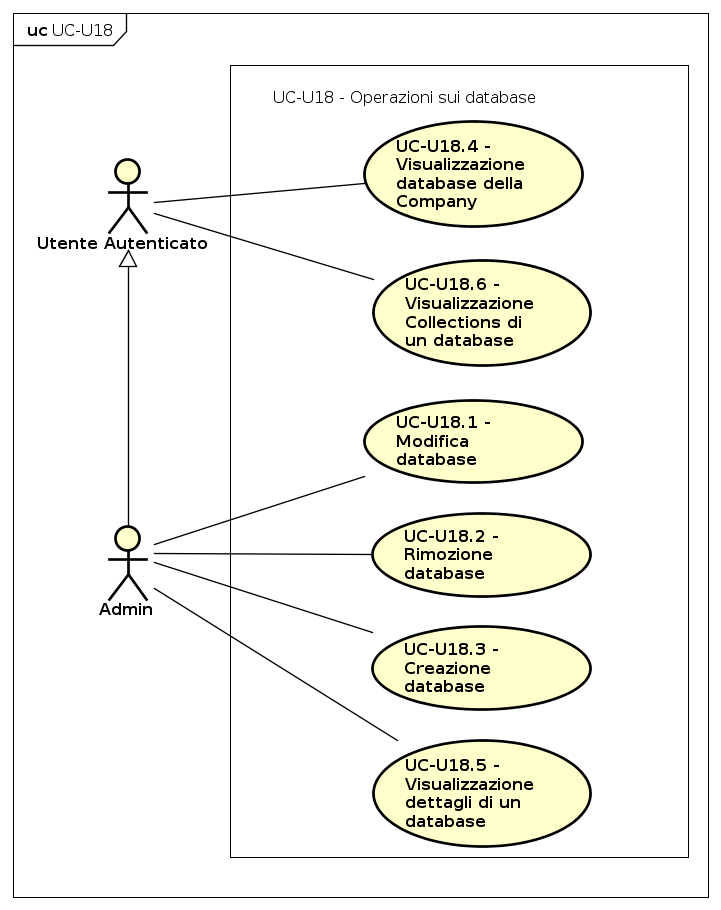
\includegraphics[width=12cm]{res/img/UCUtenti/UCUtenteA/UC-U18-OperazioniDatabase/UC-U18-OperazioniDatabase.png}
      \caption{UC-U18 - Operazioni sui database}
      \end{center} 
    \end{figure}    
    
    %Tabella 
    \begin{center}
      \bgroup
      \def\arraystretch{1.8}     
      \begin{longtable}{  p{3.5cm} | p{8cm} } 
        
        \hline
        \multicolumn{2}{ | c | }{ \cellcolor[gray]{0.9} \textbf{UC-U18 - Operazioni sui database}} \\ 
        \hline
        
        \textbf{Attori Primari} & Utente Autenticato \\ 
        \textbf{Scopo e Descrizione} & L'Utente Autenticato può visualizzare la lista dei database ai quali ha accesso. L'Admin può gestire i database della sua Company. In particolare può aggiungere, rimuovere o modificare un database, e visualizzare i dettagli di un database a scelta. \\ 
        
        \textbf{Precondizioni}  & L’applicazione è funzionante e pronta all'uso. L'utente autenticato ha visualizzato la
        pagina di gestione dei database. \\ 
        
        \textbf{Postcondizioni} & L'applicazione ha eseguito le azioni richieste dall'utente. \\ 
        \textbf{Scenario principale} & 1. L'Utente Autenticato visualizza i database ai quali ha accesso. (UC-U18.4)
        
2. L'Utente Autenticato visualizza le Collections di un database alle quali ha accesso (UC-U18.6)
        
3. L'Admin modifica un database. (UC-U18.1)

4. L'Admin rimuove un database. (UC-U18.2)

5. L'Admin aggiunge un database. (UC-U18.3)

6. L'Admin visualizza i dettagli di un un database. (UC-U18.5) \\
      \end{longtable}
      \egroup
    \end{center} 
    
\subsubsection{Modifica di un database}

    \begin{figure}[H]
      \begin{center}
        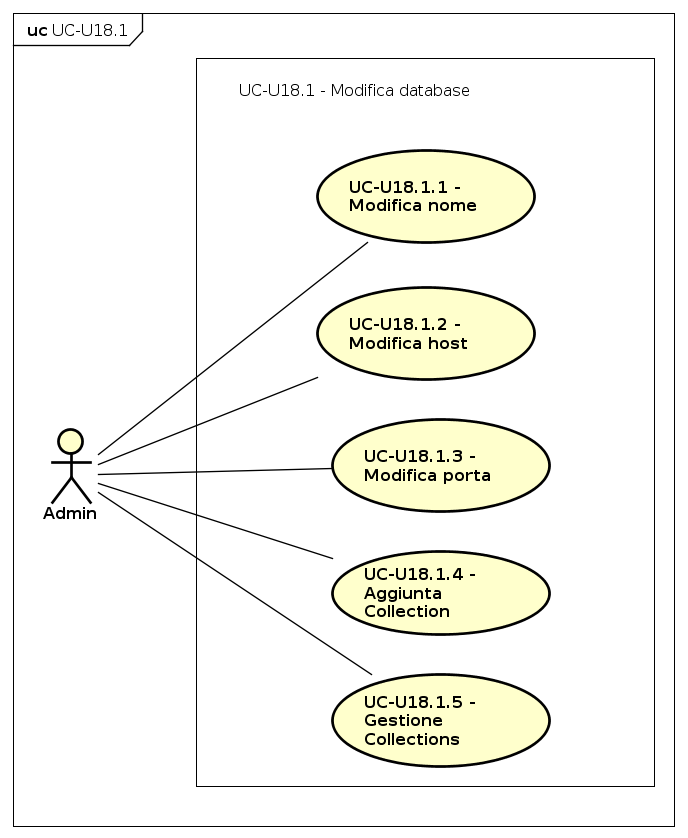
\includegraphics[width=12cm]{res/img/UCUtenti/UCUtenteA/UC-U18-OperazioniDatabase/UC-U18.1-ModificaDatabase.png}
      \caption{UC-U18.1 - Modifica di un database}
      \end{center} 
    \end{figure}    
    
    %Tabella 
    \begin{center}
      \bgroup
      \def\arraystretch{1.8}     
      \begin{longtable}{  p{3.5cm} | p{8cm} } 
        
        \hline
        \multicolumn{2}{ | c | }{ \cellcolor[gray]{0.9} \textbf{UC-U18.1 - Modifica di un database}} \\ 
        \hline
        
        \textbf{Attori Primari} & Admin \\ 
        \textbf{Scopo e Descrizione} & L'Admin può modificare i dati di connessione ad un database e le collections ad esso collegate. \\ 
        
        \textbf{Precondizioni}  & L’applicazione è funzionante e pronta all'uso. L'Admin ha visualizzato la
        pagina di modifica del database. \\ 
        
        \textbf{Postcondizioni} & L'applicazione ha eseguito le azioni richieste dall'utente. \\ 
        \textbf{Scenario principale} & 1. L'Admin inserisce il nome del database. (UC-U18.1.1)
        
2. L'Admin inserisce l'host del database. (UC-U18.1.2)

3. L'Admin inserisce la porta di accesso del database. (UC-U18.1.3)

4. L'Admin aggiunge una Collection al database. (UC-U18.1.4)

5. L'Admin modifica una Collection del database. (UC-U18.1.5) \\
      \end{longtable}
      \egroup
    \end{center} 
    
\subsubsection{Inserimento Nome Database}

    %Tabella 
    \begin{center}
      \bgroup
      \def\arraystretch{1.8}     
      \begin{longtable}{  p{3.5cm} | p{8cm} } 
        
        \hline
        \multicolumn{2}{ | c | }{ \cellcolor[gray]{0.9} \textbf{UC-U18.1.1 - Inserimento nome database}} \\ 
        \hline
        
        \textbf{Attori Primari} & Admin \\ 
        \textbf{Scopo e Descrizione} & L'Admin inserisce il nuovo nome del database. \\ 
        
        \textbf{Precondizioni}  & L'Admin ha visualizzato la pagina di modifica del database. \\ 
        
        \textbf{Postcondizioni} & L'Admin ha inserito il nuovo nome del database. \\ 
      \end{longtable}
      \egroup
    \end{center}    

\subsubsection{Inserimento Host Database}

    %Tabella 
    \begin{center}
      \bgroup
      \def\arraystretch{1.8}     
      \begin{longtable}{  p{3.5cm} | p{8cm} } 
        
        \hline
        \multicolumn{2}{ | c | }{ \cellcolor[gray]{0.9} \textbf{UC-U18.1.2 - Inserimento host database}} \\ 
        \hline
        
        \textbf{Attori Primari} & Admin \\ 
        \textbf{Scopo e Descrizione} & L'Admin inserisce il nuovo host del database. \\ 
        
        \textbf{Precondizioni}  & L'Admin ha visualizzato la pagina di modifica del database. \\ 
        
        \textbf{Postcondizioni} & L'Admin ha inserito il nuovo host del database. \\ 
      \end{longtable}
      \egroup
    \end{center}
    
\subsubsection{Inserimento Porta Database}

    %Tabella 
    \begin{center}
      \bgroup
      \def\arraystretch{1.8}     
      \begin{longtable}{  p{3.5cm} | p{8cm} } 
        
        \hline
        \multicolumn{2}{ | c | }{ \cellcolor[gray]{0.9} \textbf{UC-U18.1.3 - Inserimento porta database}} \\ 
        \hline
        
        \textbf{Attori Primari} & Admin \\ 
        \textbf{Scopo e Descrizione} & L'Admin inserisce la nuova porta del database. \\ 
        
        \textbf{Precondizioni}  & L'Admin ha visualizzato la pagina di modifica del database. \\ 
        
        \textbf{Postcondizioni} & L'Admin ha inserito la nuova porta del database. \\ 
      \end{longtable}
      \egroup
    \end{center}
    
\subsubsection{Aggiunta Collection ad un database esistente}

    \begin{figure}[H]
      \begin{center}
        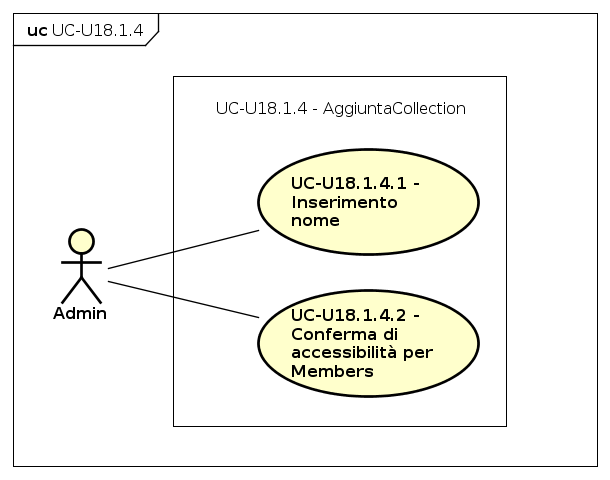
\includegraphics[width=12cm]{res/img/UCUtenti/UCUtenteA/UC-U18-OperazioniDatabase/UC-U18.1.4-AggiuntaCollection.png}
      \caption{UC-U18.1.4 - Aggiunta di una Collection ad un database esistente}
      \end{center} 
    \end{figure}    
    
    %Tabella 
    \begin{center}
      \bgroup
      \def\arraystretch{1.8}     
      \begin{longtable}{  p{3.5cm} | p{8cm} } 
        
        \hline
        \multicolumn{2}{ | c | }{ \cellcolor[gray]{0.9} \textbf{UC-U18.1.4 - Aggiunta Collection ad un database esistente}} \\ 
        \hline
        
        \textbf{Attori Primari} & Admin \\ 
        \textbf{Scopo e Descrizione} & L'Admin può aggiungere una Collection ad un database esistente. \\ 
        
        \textbf{Precondizioni}  & L’applicazione è funzionante e pronta all'uso. L'Admin ha visualizzato la
        pagina di aggiunta della Collection. \\ 
        
        \textbf{Postcondizioni} & L'applicazione ha eseguito le azioni richieste dall'utente. \\ 
        \textbf{Scenario principale} & 1. L'Admin inserisce il nome della Collection. (UC-U18.1.4.1)
        
2. L'Admin decide se la Collection è accessibile ai Member. (UC-U18.1.4.2) \\
      \end{longtable}
            \egroup
          \end{center}

\subsubsection{Inserimento nome nuova Collection}

    %Tabella 
    \begin{center}
      \bgroup
      \def\arraystretch{1.8}     
      \begin{longtable}{  p{3.5cm} | p{8cm} } 
        
        \hline
        \multicolumn{2}{ | c | }{ \cellcolor[gray]{0.9} \textbf{UC-U18.1.4.1 - Inserimento nome Collection}} \\ 
        \hline
        
        \textbf{Attori Primari} & Admin \\ 
        \textbf{Scopo e Descrizione} & L'Admin inserisce il nome della Collection. \\ 
        
        \textbf{Precondizioni}  & L'Admin ha visualizzato la pagina di inserimento della Collection. \\ 
        
        \textbf{Postcondizioni} & L'Admin ha inserito il nuovo nome della Collection. \\ 
      \end{longtable}
      \egroup
    \end{center}

\subsubsection{Inserimento accessibilità per Members per nuova Collection}

    %Tabella 
    \begin{center}
      \bgroup
      \def\arraystretch{1.8}     
      \begin{longtable}{  p{3.5cm} | p{8cm} } 
        
        \hline
        \multicolumn{2}{ | c | }{ \cellcolor[gray]{0.9} \textbf{UC-U18.1.4.2 - Inserimento accessibilità per Members}} \\ 
        \hline
        
        \textbf{Attori Primari} & Admin \\ 
        \textbf{Scopo e Descrizione} & L'Admin decide se la Collection sarà accessibile da Members. \\ 
        
        \textbf{Precondizioni}  & L'Admin ha visualizzato la pagina di inserimento della Collection. \\ 
        
        \textbf{Postcondizioni} & L'Admin ha deciso se la Collection sarà accessibile da Members. \\ 
      \end{longtable}
      \egroup
    \end{center}
    
\subsubsection{Gestione Collections di un database esistente}

    \begin{figure}[H]
      \begin{center}
        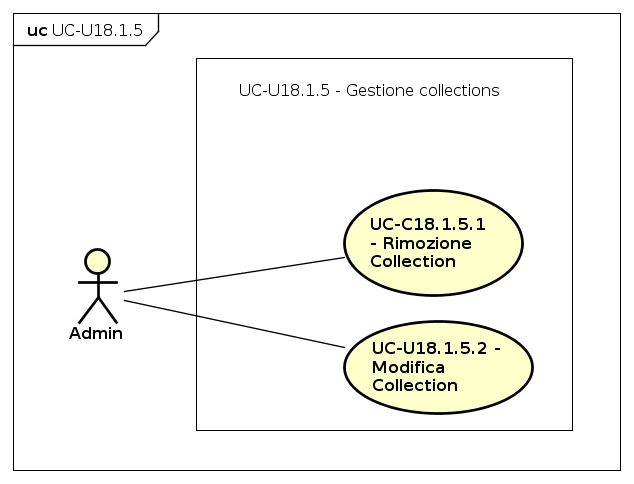
\includegraphics[width=12cm]{res/img/UCUtenti/UCUtenteA/UC-U18-OperazioniDatabase/UC-U18.1.5-GestioneCollections.png}
      \caption{UC-U18.1.5 - Gestione Collections di un database esistente}
      \end{center} 
    \end{figure}    
    
    %Tabella 
    \begin{center}
      \bgroup
      \def\arraystretch{1.8}     
      \begin{longtable}{  p{3.5cm} | p{8cm} } 
        
        \hline
        \multicolumn{2}{ | c | }{ \cellcolor[gray]{0.9} \textbf{UC-U18.1.5 - Gestione Collections di un database esistente}} \\ 
        \hline
        
        \textbf{Attori Primari} & Admin \\ 
        \textbf{Scopo e Descrizione} & L'Admin può gestire le Collections di un database esistente. \\ 
        
        \textbf{Precondizioni}  & L’applicazione è funzionante e pronta all'uso. L'Admin ha visualizzato la
        pagina di gestione delle Collections. \\ 
        
        \textbf{Postcondizioni} & L'applicazione ha eseguito le azioni richieste dall'utente. \\ 
        \textbf{Scenario principale} & 1. L'Admin rimuove una Collection. (UC-U18.1.5.1)
        
2. L'Admin modifica una Collection. (UC-U18.1.5.2) \\
      \end{longtable}
            \egroup
          \end{center}
          
\subsubsection{Rimozione Collection}

    %Tabella 
    \begin{center}
      \bgroup
      \def\arraystretch{1.8}     
      \begin{longtable}{  p{3.5cm} | p{8cm} } 
        
        \hline
        \multicolumn{2}{ | c | }{ \cellcolor[gray]{0.9} \textbf{UC-U18.1.5.2.1 - Rimozione Collection}} \\ 
        \hline
        
        \textbf{Attori Primari} & Admin \\ 
        \textbf{Scopo e Descrizione} & L'Admin rimuove una Collection. \\ 
        
        \textbf{Precondizioni}  & L'Admin ha visualizzato la pagina di gestione delle Collections. \\ 
        
        \textbf{Postcondizioni} & L'Admin ha rimosso la Collection. \\ 
      \end{longtable}
      \egroup
    \end{center}

\subsubsection{Modifica Collection di un database esistente}

    \begin{figure}[H]
      \begin{center}
        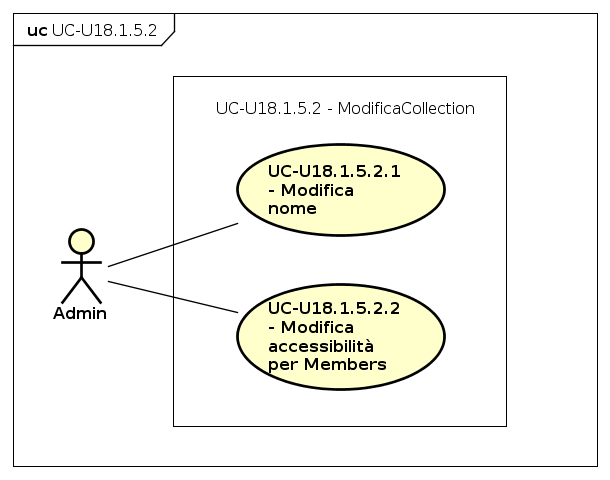
\includegraphics[width=12cm]{res/img/UCUtenti/UCUtenteA/UC-U18-OperazioniDatabase/UC-U18.1.5.2-ModificaCollection.png}
      \caption{UC-U18.1.5.2 - Modifica Collection di un database esistente}
      \end{center} 
    \end{figure}    
    
    %Tabella 
    \begin{center}
      \bgroup
      \def\arraystretch{1.8}     
      \begin{longtable}{  p{3.5cm} | p{8cm} } 
        
        \hline
        \multicolumn{2}{ | c | }{ \cellcolor[gray]{0.9} \textbf{UC-U18.1.5.2.2 - Modifica Collection di un database esistente}} \\ 
        \hline
        
        \textbf{Attori Primari} & Admin \\ 
        \textbf{Scopo e Descrizione} & L'Admin può modificare una Collection di un database esistente. \\ 
        
        \textbf{Precondizioni}  & L’applicazione è funzionante e pronta all'uso. L'Admin ha visualizzato la
        pagina di modifica della Collection. \\ 
        
        \textbf{Postcondizioni} & L'applicazione hamodificato la Collection. \\ 
        \textbf{Scenario principale} & 1. L'Admin inserisce il nome della Colelction. (UC-U18.1.5.2.2.1)
        
2. L'Admin decide se la Collection sarà accessibile ai Members. (UC-U18.1.5.2.2.2) \\
      \end{longtable}
            \egroup
          \end{center}
          
\subsubsection{Modifica nome Collection}

    %Tabella 
    \begin{center}
      \bgroup
      \def\arraystretch{1.8}     
      \begin{longtable}{  p{3.5cm} | p{8cm} } 
        
        \hline
        \multicolumn{2}{ | c | }{ \cellcolor[gray]{0.9} \textbf{UC-U18.1.5.2.2.1 - Inserimento nome Collection}} \\ 
        \hline
        
        \textbf{Attori Primari} & Admin \\ 
        \textbf{Scopo e Descrizione} & L'Admin inserisce il nome della Collection. \\ 
        
        \textbf{Precondizioni}  & L'Admin ha visualizzato la pagina di inserimento della Collection. \\ 
        
        \textbf{Postcondizioni} & L'Admin ha inserito il nuovo nome della Collection. \\ 
      \end{longtable}
      \egroup
    \end{center}

\subsubsection{Modifica accessibilità per Members}

    %Tabella 
    \begin{center}
      \bgroup
      \def\arraystretch{1.8}     
      \begin{longtable}{  p{3.5cm} | p{8cm} } 
        
        \hline
        \multicolumn{2}{ | c | }{ \cellcolor[gray]{0.9} \textbf{UC-U18.1.5.2.2.2 - Inserimento accessibilità per Members}} \\ 
        \hline
        
        \textbf{Attori Primari} & Admin \\ 
        \textbf{Scopo e Descrizione} & L'Admin decide se la Collection sarà accessibile da Members. \\ 
        
        \textbf{Precondizioni}  & L'Admin ha visualizzato la pagina di inserimento della Collection. \\ 
        
        \textbf{Postcondizioni} & L'Admin ha deciso se la Collection sarà accessibile da Members. \\ 
      \end{longtable}
      \egroup
    \end{center}
    
\subsubsection{Rimozione database}

    %Tabella 
    \begin{center}
      \bgroup
      \def\arraystretch{1.8}     
      \begin{longtable}{  p{3.5cm} | p{8cm} } 
        
        \hline
        \multicolumn{2}{ | c | }{ \cellcolor[gray]{0.9} \textbf{UC-U18.2 - Rimozione database}} \\ 
        \hline
        
        \textbf{Attori Primari} & Admin \\ 
        \textbf{Scopo e Descrizione} & L'Admin rimuove un database. \\ 
        
        \textbf{Precondizioni}  & L'Admin ha visualizzato la pagina di gestione dei database. \\ 
        
        \textbf{Postcondizioni} & L'Admin ha rimosso il database. \\ 
      \end{longtable}
      \egroup
    \end{center}

\subsubsection{Aggiunta di un database}

    \begin{figure}[H]
      \begin{center}
        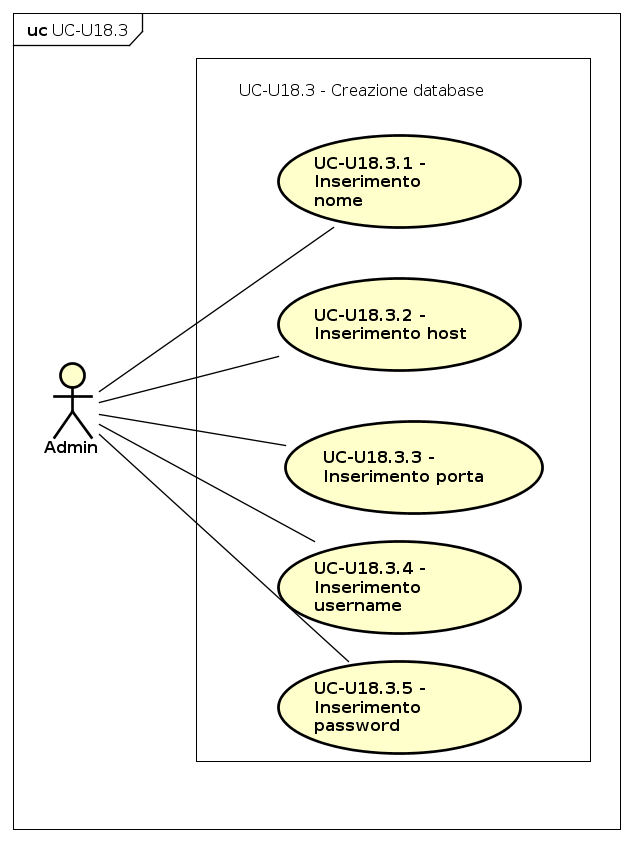
\includegraphics[width=12cm]{res/img/UCUtenti/UCUtenteA/UC-U18-OperazioniDatabase/UC-U18.3-CreazioneDatabase.png}
      \caption{UC-U18.3 - Aggiunta di un database}
      \end{center} 
    \end{figure}    
    
    %Tabella 
    \begin{center}
      \bgroup
      \def\arraystretch{1.8}     
      \begin{longtable}{  p{3.5cm} | p{8cm} } 
        
        \hline
        \multicolumn{2}{ | c | }{ \cellcolor[gray]{0.9} \textbf{UC-U18.1 - Modifica di un database}} \\ 
        \hline
        
        \textbf{Attori Primari} & Admin \\ 
        \textbf{Scopo e Descrizione} & L'Admin può modificare i dati di connessione ad un database e le collections ad esso collegate. \\ 
        
        \textbf{Precondizioni}  & L’applicazione è funzionante e pronta all'uso. L'Admin ha visualizzato la
        pagina di modifica del database. \\ 
        
        \textbf{Postcondizioni} & L'applicazione ha eseguito le azioni richieste dall'utente. \\ 
        \textbf{Scenario principale} & 1. L'Admin inserisce il nome del database. (UC-U18.3.1)
        
2. L'Admin inserisce l'host del database. (UC-U18.3.2)

3. L'Admin inserisce la porta di accesso del database. (UC-U18.3.3)

4. L'Admin aggiunge una Collection al database. (UC-U18.3.4)  \\
      \end{longtable}
      \egroup
    \end{center} 
    
\subsubsection{Inserimento Nome Database}

    %Tabella 
    \begin{center}
      \bgroup
      \def\arraystretch{1.8}     
      \begin{longtable}{  p{3.5cm} | p{8cm} } 
        
        \hline
        \multicolumn{2}{ | c | }{ \cellcolor[gray]{0.9} \textbf{UC-U18.3.1 - Inserimento nome database}} \\ 
        \hline
        
        \textbf{Attori Primari} & Admin \\ 
        \textbf{Scopo e Descrizione} & L'Admin inserisce il nuovo nome del database. \\ 
        
        \textbf{Precondizioni}  & L'Admin ha visualizzato la pagina di creazione del database. \\ 
        
        \textbf{Postcondizioni} & L'Admin ha inserito il nome del database. \\ 
      \end{longtable}
      \egroup
    \end{center}    

\subsubsection{Inserimento Host Database}

    %Tabella 
    \begin{center}
      \bgroup
      \def\arraystretch{1.8}     
      \begin{longtable}{  p{3.5cm} | p{8cm} } 
        
        \hline
        \multicolumn{2}{ | c | }{ \cellcolor[gray]{0.9} \textbf{UC-U18.3.2 - Inserimento host database}} \\ 
        \hline
        
        \textbf{Attori Primari} & Admin \\ 
        \textbf{Scopo e Descrizione} & L'Admin inserisce il nuovo host del database. \\ 
        
        \textbf{Precondizioni}  & L'Admin ha visualizzato la pagina di creazione del database. \\ 
        
        \textbf{Postcondizioni} & L'Admin ha inserito l'host del database. \\ 
      \end{longtable}
      \egroup
    \end{center}
    
\subsubsection{Inserimento Porta Database}

    %Tabella 
    \begin{center}
      \bgroup
      \def\arraystretch{1.8}     
      \begin{longtable}{  p{3.5cm} | p{8cm} } 
        
        \hline
        \multicolumn{2}{ | c | }{ \cellcolor[gray]{0.9} \textbf{UC-U18.3.3 - Inserimento porta database}} \\ 
        \hline
        
        \textbf{Attori Primari} & Admin \\ 
        \textbf{Scopo e Descrizione} & L'Admin inserisce la nuova porta del database. \\ 
        
        \textbf{Precondizioni}  & L'Admin ha visualizzato la pagina di creazione del database. \\ 
        
        \textbf{Postcondizioni} & L'Admin ha inserito la porta del database. \\ 
      \end{longtable}
      \egroup
    \end{center}
    
\subsubsection{Aggiunta Collection ad un nuovo database}

    \begin{figure}[H]
      \begin{center}
        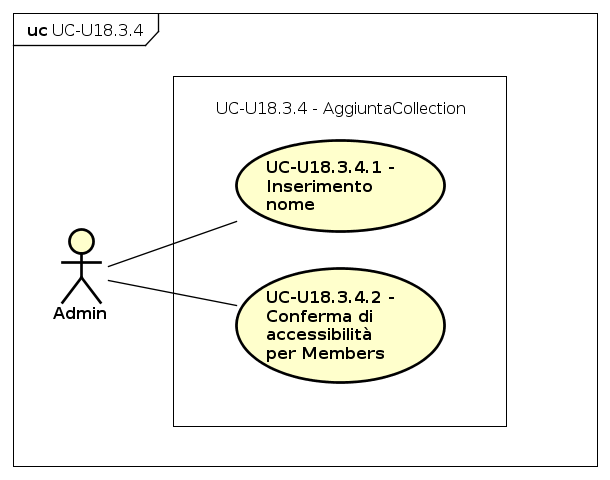
\includegraphics[width=12cm]{res/img/UCUtenti/UCUtenteA/UC-U18-OperazioniDatabase/UC-U18.3.4-AggiuntaCollection.png}
      \caption{UC-U18.3.4 - Aggiunta di una Collection ad un nuovo database}
      \end{center} 
    \end{figure}    
    
    %Tabella 
    \begin{center}
      \bgroup
      \def\arraystretch{1.8}     
      \begin{longtable}{  p{3.5cm} | p{8cm} } 
        
        \hline
        \multicolumn{2}{ | c | }{ \cellcolor[gray]{0.9} \textbf{UC-U18.3.4 - Aggiunta Collection ad un nuovo database}} \\ 
        \hline
        
        \textbf{Attori Primari} & Admin \\ 
        \textbf{Scopo e Descrizione} & L'Admin può aggiungere una Collection ad un nuovo database. \\ 
        
        \textbf{Precondizioni}  & L’applicazione è funzionante e pronta all'uso. L'Admin ha visualizzato la
        pagina di aggiunta della Collection. \\ 
        
        \textbf{Postcondizioni} & L'applicazione ha eseguito le azioni richieste dall'utente. \\ 
        \textbf{Scenario principale} & 1. L'Admin inserisce il nome della Collection. (UC-U18.3.4.1)
        
2. L'Admin decide se la Collection è accessibile ai Member. (UC-U18.3.4.2) \\
      \end{longtable}
            \egroup
          \end{center}

\subsubsection{Inserimento nome Collection}

    %Tabella 
    \begin{center}
      \bgroup
      \def\arraystretch{1.8}     
      \begin{longtable}{  p{3.5cm} | p{8cm} } 
        
        \hline
        \multicolumn{2}{ | c | }{ \cellcolor[gray]{0.9} \textbf{UC-U18.3.4.1 - Inserimento nome Collection}} \\ 
        \hline
        
        \textbf{Attori Primari} & Admin \\ 
        \textbf{Scopo e Descrizione} & L'Admin inserisce il nome della Collection. \\ 
        
        \textbf{Precondizioni}  & L'Admin ha visualizzato la pagina di inserimento della Collection. \\ 
        
        \textbf{Postcondizioni} & L'Admin ha inserito il nome della Collection. \\ 
      \end{longtable}
      \egroup
    \end{center}

\subsubsection{Inserimento accessibilità per Members per Collection}

    %Tabella 
    \begin{center}
      \bgroup
      \def\arraystretch{1.8}     
      \begin{longtable}{  p{3.5cm} | p{8cm} } 
        
        \hline
        \multicolumn{2}{ | c | }{ \cellcolor[gray]{0.9} \textbf{UC-U18.3.4.2 - Inserimento accessibilità per Members}} \\ 
        \hline
        
        \textbf{Attori Primari} & Admin \\ 
        \textbf{Scopo e Descrizione} & L'Admin decide se la Collection sarà accessibile da Members. \\ 
        
        \textbf{Precondizioni}  & L'Admin ha visualizzato la pagina di inserimento della Collection. \\ 
        
        \textbf{Postcondizioni} & L'Admin ha deciso se la Collection sarà accessibile da Members. \\ 
      \end{longtable}
      \egroup
    \end{center}
    
\subsubsection{Visualizzazione dei database della Company}

    %Tabella 
    \begin{center}
      \bgroup
      \def\arraystretch{1.8}     
      \begin{longtable}{  p{3.5cm} | p{8cm} } 
        
        \hline
        \multicolumn{2}{ | c | }{ \cellcolor[gray]{0.9} \textbf{UC-U18.4 - Visualizzazione dei database della Company}} \\ 
        \hline
        
        \textbf{Attori Primari} & Utente Autenticato \\ 
        \textbf{Scopo e Descrizione} & L'Utente Autenticato visualizza i database ai quali ha accesso. \\ 
        
        \textbf{Precondizioni}  & L'Utente Autenticato ha visualizzato la pagina di gestione dei database. \\ 
        
        \textbf{Postcondizioni} & L'Utente Autenticato ha visualizzato i database ai quali ha accesso. \\ 
      \end{longtable}
      \egroup
    \end{center}
    
\subsubsection{Visualizzazione dettagli di un database}

    %Tabella 
    \begin{center}
      \bgroup
      \def\arraystretch{1.8}     
      \begin{longtable}{  p{3.5cm} | p{8cm} } 
        
        \hline
        \multicolumn{2}{ | c | }{ \cellcolor[gray]{0.9} \textbf{UC-U18.5 - Visualizzazione dettagli di un database}} \\ 
        \hline
        
        \textbf{Attori Primari} & Admin \\ 
        \textbf{Scopo e Descrizione} & L'Admin visualizza i dettagli di un database. \\ 
        
        \textbf{Precondizioni}  & L'Admin ha visualizzato la pagina di gestione dei database. \\ 
        
        \textbf{Postcondizioni} & L'Admin ha visualizzato i dettagli di un database. \\ 
      \end{longtable}
      \egroup
    \end{center}
    
\subsubsection{Visualizzazione Collections}

    %Tabella 
        \begin{center}
          \bgroup
          \def\arraystretch{1.8}     
          \begin{longtable}{  p{3.5cm} | p{8cm} } 
            
            \hline
            \multicolumn{2}{ | c | }{ \cellcolor[gray]{0.9} \textbf{UC-U18.6 - Visualizzazione delle Collections di un database}} \\ 
            \hline
            
            \textbf{Attori Primari} & Utente Autenticato \\ 
            \textbf{Scopo e Descrizione} & L'Utente Autenticato visualizza le Collections di un database alle quali ha accesso. \\ 
            
            \textbf{Precondizioni}  & L'Utente Autenticato ha visualizzato la pagina di gestione dei database. \\ 
            
            \textbf{Postcondizioni} & L'Utente Autenticato ha visualizzato le Collections di un database alle quali ha accesso. \\ 
          \end{longtable}
          \egroup
        \end{center}
    
\subsubsection{Visualizzazione di un messaggio di errore per violazione dei permessi durante la gestione dei database}
    
        %Tabella 
                \begin{center}
                  \bgroup
                  \def\arraystretch{1.8}     
                  \begin{longtable}{  p{3.5cm} | p{8cm} } 
                    
                    \hline
                    \multicolumn{2}{ | c | }{ \cellcolor[gray]{0.9} \textbf{UC-U19 - Visualizzazione di messaggio di errore per violazione dei permessi}} \\ 
                    \hline
                    
                    \textbf{Attori Primari} & Utente autenticato \\ 
                    \textbf{Scopo e Descrizione} & L’utente autenticato visualizza un messaggio di errore nel tentativo di gestire i database.\\ 
                    
                    \textbf{Precondizioni}  & L'utente autenticato ha eseguito un'operazione sui database per la quale non dispone dei permessi. \\ 
                    
                    \textbf{Postcondizioni} & L'utente autenticato ha visualizzato il messaggio di errore. \\ 
                  \end{longtable}
                  \egroup
                \end{center}
\newpage

